
%  Beamer Style
\documentclass[xcolor={dvipsnames,rgb}]{beamer}

% \usepackage{enumitem}
% \includeonlyframes{current}
% \includeonlyframes{semantics,semantics2}

\usepackage{appendixnumberbeamer}

\usepackage{lmodern}
\usepackage[utf8]{inputenc}
\relax% Beamer Theme Customization...
    % \usetheme{default}
    \usetheme{Boadilla}
    % \ProcessOptionsBeamer
    % \useinnertheme[shadow]{rounded}
    \setbeamertemplate{blocks}[rounded][shadow=false]

    \setbeamertemplate{footline}
    {
      \leavevmode%
      \hbox{%
      \begin{beamercolorbox}[wd=.3\paperwidth,ht=2.25ex,dp=1ex,center]{author in head/foot}%
        \usebeamerfont{author in head/foot}\insertshortauthor
      \end{beamercolorbox}%
      \begin{beamercolorbox}[wd=.6\paperwidth,ht=2.25ex,dp=1ex,center]{title in head/foot}%
        \usebeamerfont{title in head/foot}\insertshorttitle
      \end{beamercolorbox}%
      \begin{beamercolorbox}[wd=.1\paperwidth,ht=2.25ex,dp=1ex,center]{date in head/foot}%
        \insertframenumber{} / \inserttotalframenumber\hspace*{1ex}
      \end{beamercolorbox}}%
      \vskip0pt%
    }

	\setbeamersize{description width=0.57cm}
	\usefonttheme[stillsansserifsmall]{serif}
		% \usefonttheme{structuresmallcapsserif}
	\usefonttheme[onlylarge]{structuresmallcapsserif}
		% \usefonttheme[onlymath]{serif}
		% \usefonttheme[onlysmall]{structurebold}
	\setbeamerfont{item}{series=\bfseries}
    \setbeamerfont{subsection in toc}{size=\small}
		% \setbeamerfont{section in toc}{size=\normalsize,series=\bfseries,shape=\upshape}
		\setbeamerfont{section in toc}{size=\normalsize}
	\setbeamerfont{block title}{series=\bfseries}
	% \setbeamerfont{title}{family=\rmfamily}

	\relax%%% color definitions %%...
		\colorlet{structurecolor}{RoyalPurple!50!black}
		\colorlet{alertcolor}{YellowOrange}
			% \colorlet{alertcolor}{structurecolor>wheel,1,3}
		\colorlet{benchcolor1}{Emerald!85!black}
			% \colorlet{benchcolor1}{structurecolor>wheel,2,3}
		\colorlet{benchcolor2}{YellowOrange!25!magenta}
	\usecolortheme[named=structurecolor]{structure}
		% \usecolortheme{beaver}
		% \setbeamercolor*{palette primary}{bg=color1, fg = green}
		% \setbeamercolor*{palette secondary}{bg=color2, fg = green}
		% \setbeamercolor*{palette tertiary}{bg=color3, fg = green}
		% \setbeamercolor*{palette quaternary}{bg=color4, fg = green}
		% \makeatletter
		% \definecolor{beamer@blendedblue}{rgb}{0.2,0.2,0.7}
		% \colorlet{beamer@blendedblue}{color2}
		% \makeatother
	\setbeamercolor{description item}{bg={structurecolor!20!white}}
	% \setbeamercolor{alerted text}{fg=alertcolor!85!red}
	\setbeamercolor{alerted text}{fg=alertcolor}
    \setbeamertemplate{navigation symbols}{}
    
    \makeatletter
    \newlength\beamerleftmargin
    \setlength\beamerleftmargin{\Gm@lmargin}
    %% stolen from:
    % https://tex.stackexchange.com/questions/34458/reference-overlay-numbers-with-names
    \DeclareRobustCommand*{\savepause}[1]{\only<1>{\immediate\write\@auxout{\string\pauseentry{\the\c@framenumber}{#1}{\the\c@beamerpauses}}}}
    \newcommand*{\usepause}[1]{\@ifundefined{pauses@\the\c@framenumber @#1}{1}{\@nameuse{pauses@\the\c@framenumber @#1}}}
    \newcommand*{\pauseentry}[3]{\global\@namedef{pauses@#1@#2}{#3}}
    \makeatother
    
    \newbool{precompiledfigs}% ...
		\setbool{precompiledfigs}{false}
		% the etoolbox way, which works with beamer.
	% \setbeamercovered{dynamic}

\relax %%%%%%%%  Beamer and slide-specific macros  %%%%%%%%%%%%%%%%%%%
	\newcommand<>{\hl}[2][alertcolor]{\begingroup%
		\setbeamercolor{alerted text}{fg=#1}\alert#3{#2}\endgroup}
	\colorlet{notationcolor}{structurecolor!30}
	\colorlet{notationalertedcolor}{structurecolor!20!alertcolor!40}
    \setbeamercolor{base notation}{fg=notationcolor}
    \setbeamercolor{alerted notation}{fg=notationalertedcolor}
	% \def\notation#1{\!\hl[notationcolor]{#1$\quad$}}
    \setbeamertemplate{alerted text begin}{
        % Set the notation color to alerted notation
        \setbeamercolor{notation}{use={alerted notation},%
            fg=alerted notation.fg,bg=alerted notation.bg}%
        %... and set the local structure to alerted text.
        \setbeamercolor{local structure}{use={alerted text},%
            fg=alerted text.fg,bg=alerted text.bg}}
    \setbeamertemplate{alerted text end}{%
        % probably no need to reset, because dying scope will reset the notation color.
        % \setbeamercolor{notation}{fg=base notation.fg, bg=base notation.bg}
    }
    % \setbeamercolor{notation}{parent={alerted text,normal text}}
	\newcommand{\notation}[1]{%
        {\usebeamercolor{notation}%
        \!\color{fg}#1$\quad$}}
        
	% \newcommand<>{\alertwith}[2]{\begingroup\only#3{\setbeamercolor{alerted text}{fg=#1}}#2\endgroup} % DOESN'T WORK THIS WAY
	\newenvironment{localfocusenv}{\only{\setbeamercolor{local structure}{fg=alertcolor}}}{}
	% \newenvironment<>{hidemeenv}{%
	% 	\only#1{\setbeamercolor{alerted text}{fg=black!60}}%
	% 	\begingroup\begin{alertenv}#1%
	% 	}{\end{alertenv}\endgroup}
	\newenvironment<>{hidemeenv}{%
        \begingroup\only#1{%
        %     \setbeamercolor{alerted text}{use={alerted text,background canvas},%
        %         fg=alerted text.fg!30!background canvas.bg}%
            \setbeamercolor{faded text}{%use={background canvas},%
                fg=normal text.fg!25!background canvas.bg}%
            \setbeamercolor{local structure}{use={faded text},fg=faded text.fg}%
            \setbeamercolor{notation}{use={base notation},fg=base notation.fg!40!background canvas.bg}
            \setbeamercolor{alerted notation}{fg=notationalertedcolor!30!background canvas.bg}
            \usebeamercolor[fg]{faded text}
        }}{\endgroup}
    \newenvironment<>{catblock}[1]{%
      \setbeamercolor{block title}{fg=white,bg=blue!95!black}
      \setbeamercolor{block body}{fg=white,bg=black}
      \begin{block}#2{#1}}{\end{block}}
        
	\newenvironment<>{tikzpicture||precompiled}[2][]{
			\ifbool{precompiledfigs}{\includegraphics[width=0.8\linewidth]{figure-pdfs/#2}
				}\begingroup\only#3\begingroup\begin{tikzpicture}[#1]
		}{\end{tikzpicture}\endgroup\endgroup}
	\newcommand<>{\extra}[2][]{%
		\only#3{%
			% \tikzmark{call point};%
			\tikzro \node[inner sep=0pt,outer sep=0pt] (call point) {};%
			\begin{tikzpicture}[overlay,remember picture]
				\node[anchor=north west, inner sep=0.8em,
				 			fill=alertcolor!30!structurecolor!30!white,
							draw=structurecolor!70!black, draw opacity=0.5,
							below=1em of call point, #1]{#2};
			\end{tikzpicture}%
		}}
	\newcommand{\tikzro}[1][]{\tikz[remember picture, overlay,#1]}
	\def\Set{\mathbf{Set}}
	\makeatletter
	\newcommand{\shorteq}{%
	  \settowidth{\@tempdima}{-}% Width of hyphen
	  \resizebox{\@tempdima}{\height}{=}%
	}
	\makeatother
    %https://tex.stackexchange.com/questions/34921/how-to-overlap-images-in-a-beamer-slide
    \def\Put(#1,#2)#3{\leavevmode\makebox(0,0){\put(#1,#2){#3}}}

	% \newcommand{\tikzmark}[1][last mark]{\tikzro \node (#1){};}

%%%%%%%            Relevant part of PDG Preamble        %%%%%%%%%%%%%%%%
\usepackage{tikz}
	\usetikzlibrary{positioning,calc, arrows, shapes}

	\tikzset{AmpRep/.style={ampersand replacement=\&}}
	\tikzset{center base/.style={baseline={([yshift=-.8ex]current bounding box.center)}}}
	\tikzset{paperfig/.style={center base,scale=0.9, every node/.style={transform shape}}}

	\tikzset{dpadded/.style={rounded corners=2, inner sep=0.6em, draw, outer sep=0.2em, fill={black!50}, fill opacity=0.08, text opacity=1}}
	\tikzset{light pad/.style={outer sep=0.2em, inner sep=0.5em, draw=gray!50}}
	\tikzset{arr/.style={draw, ->, thick, shorten <=3pt, shorten >=3pt}}
	\tikzset{arr0/.style={draw, ->, thick, shorten <=0pt, shorten >=0pt}}
	\tikzset{arr1/.style={draw, ->, thick, shorten <=1pt, shorten >=1pt}}
	\tikzset{arr2/.style={draw, ->, thick, shorten <=2pt, shorten >=2pt}}

	\newcommand{\drawbb}%
		{\draw (current bounding box.south west) rectangle (current bounding box.north east);}
	\ifbool{precompiledfigs}{}{
		\usetikzlibrary{fit, decorations,shapes.geometric}
		\usetikzlibrary{tikzmark}
		\usetikzlibrary{backgrounds}
		\pgfdeclarelayer{foreground}
		\pgfsetlayers{background,main,foreground}

		\pgfdeclaredecoration{arrows}{draw}{
			\state{draw}[width=\pgfdecoratedinputsegmentlength]{%
				\path [every arrow subpath/.try] \pgfextra{%
					\pgfpathmoveto{\pgfpointdecoratedinputsegmentfirst}%
					\pgfpathlineto{\pgfpointdecoratedinputsegmentlast}%
				};
		}}

		% \tikzset{dpad0/.style={outer sep=0.05em, inner sep=0.3em, draw=gray!75, rounded corners=4, fill=black!08, fill opacity=1}}
		\tikzset{dpad0/.style={outer sep=0.05em, inner sep=0.2em, draw=gray!75, draw opacity=0.5, rounded corners=3, fill=black!18, fill opacity=0.4, text=black, text opacity=1}}
        
		\tikzset{dpad/.style args={#1}{every matrix/.append style={nodes={dpadded, #1}}}}
		\tikzset{is bn/.style={background rectangle/.style={fill=blue!35,opacity=0.3, rounded corners=5},show background rectangle}}
		% \usetikzlibrary{backgrounds}
		% \usetikzlibrary{patterns}
		\usetikzlibrary{cd}

		\tikzset{fgnode/.style={dpadded,inner sep=0.2em, circle,minimum width=2.3em},
				 factor/.style={light pad, fill=black, outer sep=0pt,draw=none}}


		\newcommand\cmergearr[5][]{
			\draw[arr,-] (#2) -- (#5) -- (#3);
			\draw[arr, shorten <=0, #1] (#5) -- (#4);
			}
		\newcommand\mergearr[4][]{
			\coordinate (center-#2#3#4) at (barycentric cs:#2=1,#3=1,#4=1.2);
			\cmergearr[#1]{#2}{#3}{#4}{center-#2#3#4}
			}
		\newcommand\cunmergearr[5][]{
			\draw[arr,-, , shorten >=0] (#2) -- (#5);
			\draw[arr, shorten <=0, #1] (#5) -- (#3);
			\draw[arr, shorten <=0, #1] (#5) -- (#4);
			}
		\newcommand\unmergearr[4][]{
			\coordinate (center-#2#3#4) at (barycentric cs:#2=1.2,#3=1,#4=1);
			\cunmergearr[#1]{#2}{#3}{#4}{center-#2#3#4}
			}


		\usetikzlibrary{matrix}
		\tikzset{toprule/.style={%
		        execute at end cell={%
		            \draw [line cap=rect,#1]
		            (\tikzmatrixname-\the\pgfmatrixcurrentrow-\the\pgfmatrixcurrentcolumn.north west) -- (\tikzmatrixname-\the\pgfmatrixcurrentrow-\the\pgfmatrixcurrentcolumn.north east);%
		        }
		    },
		    bottomrule/.style={%
		        execute at end cell={%
		            \draw [line cap=rect,#1] (\tikzmatrixname-\the\pgfmatrixcurrentrow-\the\pgfmatrixcurrentcolumn.south west) -- (\tikzmatrixname-\the\pgfmatrixcurrentrow-\the\pgfmatrixcurrentcolumn.south east);%
		        }
		    },
		    leftrule/.style={%
		        execute at end cell={%
		            \draw [line cap=rect,#1] (\tikzmatrixname-\the\pgfmatrixcurrentrow-\the\pgfmatrixcurrentcolumn.north west) -- (\tikzmatrixname-\the\pgfmatrixcurrentrow-\the\pgfmatrixcurrentcolumn.south west);%
		        }
		    },
		    rightrule/.style={%
		        execute at end cell={%
		            \draw [line cap=rect,#1] (\tikzmatrixname-\the\pgfmatrixcurrentrow-\the\pgfmatrixcurrentcolumn.north east) -- (\tikzmatrixname-\the\pgfmatrixcurrentrow-\the\pgfmatrixcurrentcolumn.south east);%
		        }
		    },
		    table with head/.style={
			    matrix of nodes,
			    row sep=-\pgflinewidth,
			    column sep=-\pgflinewidth,
			    nodes={rectangle,minimum width=2.5em, outer sep=0pt},
			    row 1/.style={toprule=thick, bottomrule},
	  	    }
			}
		\usepackage{environ}
\usepackage{xstring}

% Wow this works I'm brilliant
\def\wrapwith#1[#2;#3]{
	\expandarg\IfSubStr{#1}{,}{
		\expandafter#2{\expandarg\StrBefore{#1}{,}}
		\expandarg\StrBehind{#1}{,}[\tmp]
		\xdef\tmp{\expandafter\unexpanded\expandafter{\tmp}}
		#3
		\wrapwith{\tmp}[#2;{#3}]
	}{ \expandafter#2{#1} }
}
\def\hwrapcells#1[#2]{\wrapwith#1[#2;&]}
\def\vwrapcells#1[#2]{\wrapwith#1[#2;\\]}
\NewEnviron{mymathenv}{$\BODY$}

\newcommand{\smalltext}[1]{\text{\footnotesize#1}}
\newsavebox{\idxmatsavebox}
\def\makeinvisibleidxstyle#1#2{\phantom{\hbox{#1#2}}}
\newenvironment{idxmatphant}[4][\color{gray}\smalltext]{%
	\def\idxstyle{#1}
	\def\colitems{#3}
	\def\rowitems{#2}
	\def\phantitems{#4}
	\begin{lrbox}{\idxmatsavebox}$%$\begin{mymathenv}
	\begin{matrix}  \begin{matrix} \hwrapcells{\colitems}[\idxstyle]  \end{matrix}
		% &\vphantom{\idxstyle\colitems}
		\\[-0.05em]
		\left[
		\begin{matrix}
			\hwrapcells{\phantitems}[\expandafter\makeinvisibleidxstyle\idxstyle]  \\[-1.2em]
	}{
		\end{matrix}\right]		&\hspace{-0.8em}\begin{matrix*}[l] \vwrapcells{\rowitems}[\idxstyle] \end{matrix*}\hspace{0.1em}%
	\end{matrix}%
	$%\end{mymathenv}
	\end{lrbox}%
	\raisebox{0.75em}{\usebox\idxmatsavebox}
%	\vspace{-0.5em}
}

\newenvironment{idxmat}[3][\color{gray}\smalltext]
	{\begingroup\idxmatphant[#1]{#2}{#3}{#3}}
	{\endidxmatphant\endgroup}

\newenvironment{sqidxmat}[2][\color{gray}\smalltext]
	{\begingroup\idxmat[#1]{#2}{#2}}
	{\endidxmat\endgroup}


%%%%%%%%%%%%
% better alignment for cases
\makeatletter
\renewenvironment{cases}[1][l]{\matrix@check\cases\env@cases{#1}}{\endarray\right.}
\def\env@cases#1{%
	\let\@ifnextchar\new@ifnextchar
	\left\lbrace\def\arraystretch{1.2}%
	\array{@{}#1@{\quad}l@{}}}
\makeatother

		\tikzset{onslide/.code args={<#1>#2}{%
		  \only<#1>{\pgfkeysalso{#2}} % \pgfkeysalso doesn't change the path
			}}
		}
		\newcommand{\TODO}[1][INCOMPLETE]{{\centering\Large\color{red}$\langle$~\texttt{#1}~$\rangle$\par}}
    
    % Tikz Externalization doesn't work with beamer with all of the animations...
    % \newif\ifexternalizefigures\externalizefigurestrue
    % \ifexternalizefigures
    % 	\usetikzlibrary{external}
    % 	\tikzexternalize[prefix=tikz/]  % activate!
    % 	\fi

\usepackage{booktabs,microtype}
\usepackage{mathtools, amsfonts, nicefrac, amssymb, bbm} % mathtools loads amsmath
\usepackage{faktor}
\usepackage{amsthm,thmtools}
	% \theoremstyle{plain}
	% \let\theorem\relax
	% \newtheorem{theorem}{Theorem}%[section]
	% \newtheorem{coro}{Corollary}[theorem]
	\newtheorem{prop}[theorem]{Proposition}
	% \newtheorem{lemma}[theorem]{Lemma}
	% \newtheorem{fact}[theorem]{Fact}

	\theoremstyle{definition}
	\declaretheorem[name=Definition%,qed=$\square$,numberwithin=section
		]{defn}
	% \declaretheorem[name=Construction,qed=$\square$,sibling=defn]{constr}
	% \declaretheorem[qed=$\square$]{example}
	\theoremstyle{remark}
	\newtheorem*{remark}{Remark}
\relax % Macros (\relax is for folding)
	\let\Horig\H
	\let\H\relax
	\DeclareMathOperator{\H}{\mathrm{H}} %
	\DeclareMathOperator{\I}{\mathrm{I}} %
	\DeclareMathOperator*{\Ex}{\mathbb{E}} %
	\DeclareMathOperator*{\argmin}{arg\;min}
	\newcommand{\CI}{\mathrel{\perp\mspace{-10mu}\perp}} %
	\newcommand\mat[1]{\mathbf{#1}}
	\newcommand\Pa{\mathbf{Pa}}

	\DeclarePairedDelimiterX{\infdivx}[2]{(}{)}{#1\;\delimsize\|\;#2}
	\newcommand{\thickD}{I\mkern-8muD}
	\newcommand{\kldiv}{\thickD\infdivx}

	\newcommand{\tto}{\rightarrow\mathrel{\mspace{-15mu}}\rightarrow}

	\newcommand{\ssub}[1]{_{\!_{#1}\!}}
	\newcommand{\bp}[1][L]{\mat{p}\ssub{#1}}
	\newcommand{\V}{\mathcal V}
	\newcommand{\N}{\mathcal N}
	\newcommand{\Ed}{\mathcal E}

	\DeclareMathAlphabet{\mathdcal}{U}{dutchcal}{m}{n}
	\DeclareMathAlphabet{\mathbdcal}{U}{dutchcal}{b}{n}

	\newcommand{\dg}[1]{\mathbdcal{#1}}
	\newcommand{\pdgunit}{\mathrlap{\mathit 1} \mspace{2.3mu}\mathit 1}

	\newcommand{\IDef}[1]{\mathit{IDef}_{\!#1}}
	\newcommand\Inc{\mathit{Inc}}
	\newcommand{\PDGof}[1]{{\dg M}_{#1}}
	\newcommand{\UPDGof}[1]{{\dg N}_{#1}}
	\newcommand{\WFGof}[1]{\Psi_{{#1}}}
	\newcommand{\FGof}[1]{\Phi_{{#1}}}
	\newcommand{\Gr}{\mathcal G}
	\newcommand\GFE{\mathit{G\mkern-4mu F\mkern-4.5mu E}}

	\newcommand{\datadist}[1]{\Pr\nolimits_{#1}}
    \newcommand\xsamp{{\underline{\mat x}}}
    \newcommand\xysamp{{\underline{\mat{xy}}}}

	\newcommand{\ed}[3]{%
		\mathchoice%
		{#2\overset{\smash{\mskip-5mu\raisebox{-3pt}{${#1}$}}}{\xrightarrow{\hphantom{\scriptstyle {#1}}}} #3} %display style
		{#2\overset{\smash{\mskip-5mu\raisebox{-3pt}{$\scriptstyle {#1}$}}}{\xrightarrow{\hphantom{\scriptstyle {#1}}}} #3}% text style
		{#2\overset{\smash{\mskip-5mu\raisebox{-3pt}{$\scriptscriptstyle {#1}$}}}{\xrightarrow{\hphantom{\scriptscriptstyle {#1}}}} #3} %script style
		{#2\overset{\smash{\mskip-5mu\raisebox{-3pt}{$\scriptscriptstyle {#1}$}}}{\xrightarrow{\hphantom{\scriptscriptstyle {#1}}}} #3}} %scriptscriptstyle

	% \DeclarePairedDelimiterX{\SD}[1]{\{}{\}}{\,\llap{\delimsize\{}#1\rlap{\delimsize\}}\,}
	%better version.
	% \DeclarePairedDelimiterX{\bbr}[1]{[}{]}
	% 	{\mspace{3mu}\mathllap{\delimsize[}#1\mathrlap{\delimsize]}\mspace{3mu}}
	% \DeclarePairedDelimiterX{\aar}[1]{\langle}{\rangle}
	% 	{\mspace{3mu}\mathllap{\delimsize\langle}#1\mathrlap{\delimsize\rangle}\mspace{3mu}}
	% \DeclarePairedDelimiterXPP{\aard}[1]{}{\langle}{\rangle}{_{\!_\downarrow}}
	% 	{\mspace{-3.5mu}\delimsize\langle#1\delimsize\rangle\mspace{-3.5mu}}
    \usepackage{scalerel}
    \newcommand{\nhphantom}[2]{\sbox0{\kern-2%
    		\nulldelimiterspace$\left.\delimsize#1\vphantom{#2}\right.$}\hspace{-.97\wd0}}
    		% \nulldelimiterspace$\left.\delimsize#1%
    		% \vrule depth\dp#2 height \ht#2 width0pt\right.$}\hspace{-.97\wd0}}
	\makeatletter
	\newsavebox{\abcmycontentbox}
	\newcommand\DeclareDoubleDelim[5]{
	    \DeclarePairedDelimiterXPP{#1}[1]%
			{% box must be saved in this pre code
				\sbox{\abcmycontentbox}{\ensuremath{##1}}%
			}{#2}{#5}{}%
		    %%% Correct spacing, but doesn't work with externalize.
			% {\nhphantom{#3}{##1}\hspace{1.2pt}\delimsize#3\mathopen{}##1\mathclose{}\delimsize#4\hspace{1.2pt}\nhphantom{#4}{##1}}
			%%% Fast, but wrong spacing.
			% {\nhphantom{#3}{~}\hspace{1.2pt}\delimsize#3\mathopen{}##1\mathclose{}\delimsize#4\hspace{1.2pt}\nhphantom{#4}{~}}
			%%% with savebox.
		    {%
				\nhphantom{#3}{\usebox\abcmycontentbox}%
				\hspace{1.2pt} \delimsize#3%
				\mathopen{}\usebox{\abcmycontentbox}\mathclose{}%
				\delimsize#4\hspace{1.2pt}%
				\nhphantom{#4}{\usebox\abcmycontentbox}%
			}%
    	}
    	\makeatother
    	\DeclareDoubleDelim
    		\SD\{\{\}\}
    	\DeclareDoubleDelim
    		\bbr[[]]
	% \DeclareDoubleDelim
	% 	\aar\langle\langle\rangle\rangle
	\makeatletter
	\newsavebox{\aar@content}
	\newcommand\aar{\@ifstar\aar@one@star\aar@plain}
	\newcommand\aar@one@star{\@ifstar\aar@resize{\aar@plain*}}
	\newcommand\aar@resize[1]{\sbox{\aar@content}{#1}\scaleleftright[3ex]
		{\Biggl\langle\!\!\kern0.3pt\!\!\Biggl\langle}{\usebox{\aar@content}}
		{\Biggr\rangle\!\!\kern0.3pt\!\!\Biggr\rangle}}
	\DeclareDoubleDelim
		\aar@plain\langle\langle\rangle\rangle
	\makeatother

%Information to be included in the title page:
% \title{Probabilsitic Dependency Graphs, and Inconsistency}
\title{Probabilistic Dependency Graphs and Inconsistency}
    \subtitle{How to model, measure, and mitigate internal conflict}
	\author[Oliver~Richardson]{Oliver Richardson}
	\institute[Cornell]{Cornell University\\Department of Computer Science}
	\date{September 2021}

\AtBeginSection[]
{
  \begin{frame}<beamer>
    % \frametitle{Outline for section \thesection}
    \frametitle{Outline for Section \thesection}
		% \setlength\fboxsep{0pt}
		% \fbox{
    \begin{columns}[T]
				% \addtolength{\leftskip}{2cm}
        \column{0.45\textwidth}
				\begin{minipage}[t][0.84\textheight]{\linewidth}
				\raggedright
        \tableofcontents[currentsection,sections={1-4}]
				\end{minipage}
				
        \column{0.45\textwidth}
				\begin{minipage}[t][0.8\textheight]{\linewidth}
				\raggedright
        \tableofcontents[currentsection,sections={<5->}]
				\end{minipage}
    \end{columns}
		%}
  \end{frame}
}

\begin{document}
\frame{\titlepage}


\begin{frame}
    % First few sentences need to be about 
    % (1) ease of use
    % (2) 
    % Motivation: 
    %  Suppose you're
    The standard way of modeling an agent with uncertainty:
    
    \begin{itemize}%[noitemsep]        
            \setlength{\itemsep}{0pt}
            \setlength{\parskip}{0pt}
            \setlength{\parsep}{0pt}
        \item a probability distribution $p : \Delta W$ over worlds $W$,
        \item a utility function $u:\Omega \to \mathbb R$, some actions $A$. 
    \end{itemize}
    \medskip
    
    \begin{center}
        \begin{tikzpicture}
            \node[dpadded] (W) at (0,0) {$W$};
            \node[dpadded] (O) at (2,0) {$\Omega$};
            \node[dpadded] (A) at (0.8,1) {$A$};
            \node[dpadded] (U) at (3.8,0) {$U$};
            % 
            \draw[arr2, <-] (W) -- node[above]{$p$} ++(-1.5, 0);
            \mergearr[->>] WAO
            \draw[arr2, ->>] (O) -- node[above]{$u$}  (U);
        \end{tikzpicture}
    \end{center}
    
    % Interesting behavior arises from interactions with the environment or other agents, tricks to make computation tractable (independencies, approximation algorithms)
    % Addiction. 
    \medskip
    
    Such agents cannot have internal conflict;\\    
    {\color{gray}\hspace{1em} by construction, they have consistent beliefs and desires.}
\end{frame}

\begin{frame}
    % Rhetorical Question
		\TODO
    \begin{block}{}
        {Why build systems that can be inconsistent, if inconsistency is bad? }
    \end{block}
    
    {Why entertain the possibility of being wrong, if being wrong is bad? }
    % 
    % \begin{catblock}{}
    %     a 
    % \end{catblock}
    
    
    
    Elsewhere, computer scientists take great care to model inconsistency:
    \begin{itemize}        
        \item assertions and test cases: 
        
        \item 
        \item losses for training neural networks
            \hfill\texttt{\color{gray} (totally separate from the probabilistic model)}
    \end{itemize}
    
    % ALl of these are things you can find...
\end{frame}




\begin{frame}\frametitle{Yet Another Probabilistic Graphical Model}
	\TODO[remove slide, once intro is finished]
	
	We introduce \textit{probabilistic dependency graphs} (PDGs), a new class of graphical models
	for representing uncertainty. 
	
	\pause
	\bigskip
	{\centering\Large Why do we need another one?\par}
	
	\bigskip
	\pause
	\begin{itemize}[<+-|alert@+>]
		\item To resolve inconsistency, we must first model it.
		\item In doing so, we get much more \ldots
	\end{itemize}
\end{frame}



	\begin{frame} %%%%%%%%%%%        REVIEW OF BNS      %%%%%%%%%%%%%%%%
		\frametitle{Two aspects of Bayesian Networks (BNs)}
		\begin{description}
			\item<+->[{\color{benchcolor2!70!black}Qualitative} BN,~~$\Gr$]~\\
				an independence relation on variables
				\begin{itemize}\small
					\item {\color{gray} $X \CI_{\Gr} Y \mid \Pa(X)$, for all non-descendents $Y$ 	of $X$}
				\end{itemize}\medskip
			\item<+->[({\color{benchcolor1!80!black}Quantitative}) BN,~~$\mathcal B = (\Gr, \mat p)$]~\\
					a qualitative BN ($\Gr$) and a cpd
					$p_{\!_X}(X \mid \Pa(X))$ for each variable $X$.
					\vspace{-1.2em}
					%
					\begin{itemize} \small
						\item {\color{gray}Defines a joint distribution $\Pr_{\mathcal B}$ \hl[benchcolor2]<+>{with the independencies $\CI_\Gr$}.}
					\end{itemize}
			\end{description}
		\vspace{2em}
		\begin{center}
			\begin{tikzpicture}[paperfig]
				\begin{scope}[every node/.style={dpadded, fill opacity=1,fill=black!08, circle, inner sep=2pt, minimum size=2em, draw=gray}]
					\node (PS) at (0,0) {$\mathit{PS}$};
					\node (SH) at (1.5, 0.6) {$\mathit{SH}$};
					\node (S) at (1.5, -0.6) {$\mathit{S}$};
					\node (C) at (3, 0) {$\mathit{C}$};
					\end{scope}
				\draw[->] (PS) to (S);
				\draw[->] (PS) to (SH);
				\draw[->] (SH) to (C);
				\draw[->] (S) to (C);
				\end{tikzpicture}
			\end{center}
		\end{frame}

\section{Modeling Examples}
	\subsection{The Simplest Inconsistency}
		\newlength{\bncolwidth}
		\begin{frame} %%%%%%%%%       GUN FLOOMP: BN vs PDG       %%%%%%%%%%
			%% 1 -- Just BN
			%% 2 -- add PDG.
			%% 3 -- List appears, arbitrary new info.
			%% 4 -- list highlighted, p appears both diagrams (dashed), green box.
			%% 5 -- inconsistent PDG?
			%% 6-8 -- variants of BN w / different info. Final point visible.
			\frametitle{Simple Example: Floomps and Guns}
			% \framesubtitle{The Legality of Floomps and Guns}
			\only<1-3>{
				{\centering	Grok thinks it likely (.95) that guns are illegal,\\
				but that floomps (local slang) are legal (.90).\par}
			}
			\pause
			\colorlet{heldout}{benchcolor1!80!black}

			% \only<2->{ % Headers "BN" and "PDG"
				\vspace{1.2em}
				\begin{columns}[c]
					\Large\color{structurecolor}
					\begin{column}{.45\textwidth}\centering% Add BN to diagram
						\only<4,5>{\color{structurecolor!20}}%
						\textbf{BN}\\[-1em]
						\rule{2.2cm}{0.95pt}\end{column}
					\only<3->{ % add PDG to diagram
						% \vrule
						\begin{column}{.5\textwidth}\centering%
							\only<6->{\color{structurecolor!20}}%
							\textbf{PDG}\\[-1em]
							\rule{2.7cm}{0.95pt}\end{column}
						}
					\end{columns}
				\vspace{0.0em}
				% }

	
			\begin{columns}[c] %% (both diagrams) ...
				\setlength{\bncolwidth}{0.45\textwidth}
				\only<6->{\setlength{\bncolwidth}{0.51\textwidth}}
				\begin{column}{\bncolwidth} % BN Diagram
					% \begin{block}{BN}
						\centering
						% \hspace{-2.5em}
						\begin{tikzpicture||precompiled}{fg-BN}[AmpRep, scale=0.9]
							\def\figtabledist{0.50}
							\def\fignodedist{0.8}
							\def\figtableheight{0.32}

							%% Time to unify the notation for cpds.
							% \matrix [table with head, column 1/.style={leftrule}, anchor=south east,
							% 	 column 2/.style={rightrule}, row 2/.style={bottomrule}] at (-\figtabledist,\figtableheight) {
							% 	\vphantom{$\overline fg$} $f$ \& \vphantom{$\overline fg$}$\overline f$\\
							% 	.9 \& .1\\
							% };
							% \matrix [table with head, column 1/.style={leftrule}, anchor=south west,
							% 	 column 2/.style={rightrule}, row 2/.style={bottomrule}] at (\figtabledist,\figtableheight) {
							% 	 \vphantom{$\overline fg$}$g$ \& \vphantom{$\overline fg$}$\overline g$\\
							% 	 .05 \& .95\\
							% };
							\node[% F's cpd ...
									anchor=south east]
							 	at (-\figtabledist,\figtableheight) {%    
                                \color<6-8>{benchcolor1!70!black}
								\hspace{-1.2em}%
								\only<1-6,8>{\begin{idxmat} [\color{gray!60}\smalltext]
									{\!\!}{$f$,$\overline f$}
										.90 & .10 \\
									\end{idxmat}}%
								\only<7>{ \begin{idxmat}[\color{gray!60}\smalltext]
									{$g$,$\overline g$}{$f$,$\overline f$}
										.92 & .08 \\
										.08 & .92 \\
									\end{idxmat}\hspace{-1em}\;}%
								};
							\node[% G's cpd ...
									anchor=south west]
								at (\figtabledist,\figtableheight) {%
                                \color<6-8>{benchcolor1!70!black}
								\hspace{-1.2em}%
								\only<1-7>{\begin{idxmat}[\color{gray!60}\smalltext]
									{\!\!}{$g$,$\overline g$}
									.05 & .95 \\
									\end{idxmat}}%
								\only<8>{\begin{idxmat}[\color{gray!60}\smalltext]
									{$f$,$\overline f$}{$g$,$\overline g$}
										.92 & .08 \\
										.08 & .92 \\
									\end{idxmat}}%
								% \hspace{-0.5em}~%
								};
							\node[% F (floomp) ...
								dpadded, inner sep=0.5em, circle, fill=black!08, fill opacity=1]
								(floomp) at (-\fignodedist,0) {$F$};
							\node[% G (gun) ...
								dpadded, inner sep=0.5em, circle, fill=black!08, fill opacity=1]
								(gun) at (\fignodedist,0) {$G$};
							% \node (leftbounds) at (-3,0){};
							% \node (rightbounds) at (3,0){};

							\onslide<7,8>{ \draw[thick, ->, onslide=<8>{<-}, benchcolor2] 
								(gun) -- node[below,align=center,font=\tiny]{must\\choose\\direction} (floomp); }

							% \only<6->{\node[align=left,% show which cpds are incorporated...
							% 		rounded corners=5, inner sep=0.5em, 
							% 		fill=structurecolor!50!benchcolor1!10,
							% 		draw=structurecolor!50!benchcolor1!50] (incorporated) 
							%  		at (0,-1.5)
							% 	{ \textit{BN Contents}:\\\Large
							% 		\hspace{1em}
							% 		\hl[benchcolor1]<6,8>{$\mu\ssub F$}
							% 		\hspace{1em}
							% 		\hl[benchcolor1]<6,7>{$\mu\ssub G$}
							% 		\hspace{1em}
							% 		\hl[benchcolor1]<8>{$p$}
							% 		\hspace{1em}
							% 		\hl[benchcolor1]<7>{$p'$}
							% 	};\node[below=1em of incorporated]{};}

							\only<4-6>{		\node[text=alertcolor] at (0,+0.8){$p$??};		}
							\only<4,5>{ \fill[white,opacity=0.8] (-3, -0.8) rectangle (3,1.8); }
							\useasboundingbox (-2.7, -0.8) rectangle (2.7,1.8);
							\end{tikzpicture||precompiled}
					% \end{block}
					\vspace{-0.8em}
					\end{column}
				\only<3,4>{{\color{gray}\vrule}}
				\begin{onlyenv}<3->\begin{column}{0.95\textwidth-\bncolwidth}
					% \only<6->{{~\hspace{-2em}~}}
					% \centering
					\begin{tikzpicture||precompiled}{fg-PDG}[]
						\def\fignodedist{1.5}
						\node[% for  "1"  /  "true"  ...
							dpadded, fill=gray!20, draw=gray!70, inner sep=0.35em, outer sep=0.37em]
							(true)  at (0,1.3) {$\pdgunit$};
						\node[dpadded] (floomp) at (-\fignodedist, 0) {$F$};
						\node[dpadded] (gun) at (\fignodedist, 0) {$G$};

						\begin{pgfonlayer}{foreground}
							\draw[arr1,{onslide=<6,8>{benchcolor1!70!black}},
                                    {onslide=<7>{gray!50!white}}]
								(true.-165) -- %to[bend right=0]
									(floomp.60)
									node[pos=.5,{onslide=<6->{above left}}] (A)
										{\only<6->{$\mu\ssub F$}}
									;
							\draw[arr1,{onslide=<6,7>{benchcolor1!70!black}},
                                    {onslide=<8>{gray!50!white}}]
								(true.-15) -- %to[bend left=0]
									(gun.120)
									node[pos=.5,{onslide=<6->{above right}}] (B)
									 	{\only<6->{$\mu\ssub G$}}
									;
							\end{pgfonlayer}

						\node[, % CPT for F...
							above left=1.5em and 2.5em of A.center, anchor=center] {%
							\color<5>{alertcolor}
							\alt<6->{}{
								\hspace{-0.8em}%
								\begin{idxmat}
									[\color{gray!60}\color<5>{alertcolor!50}\smalltext]
									%[\color{black}\smalltext]
									{$\star$}{$f$, $\overline f$}
									.90 & .10 \\
								\end{idxmat}
								\hspace{-1em}~}
							};
						\node[, % CPT for G...
							above right=1.5em and 2.3em of B.center, anchor=center] {
							\color<5>{alertcolor}
							\alt<6->{}{
								\hspace{-0.8em}
								\begin{idxmat}
									[\color{gray!60}\color<5>{alertcolor!50}\smalltext]
									%[\color{black}\smalltext]
									{$\star$}{$g$, $\overline g$}
									.05 & .95 \\
								\end{idxmat}
								\hspace{-1em}~}
							};
						\only<4->{ % Show p & arrows, after initial diagrams...
							\begin{pgfonlayer}{foreground}
								\draw[arr,
										onslide=<4>{heldout, dashed},
                                        {onslide=<6,7>{gray!50!white}},
								 		{onslide=<8>{benchcolor1!70!black}},
										onslide=<5>{text=alertcolor} ]
								 	(floomp.-33) to[bend right=6] node[pos=0.65, fill=white, inner sep=2pt] (C) {$\smash{p}\vphantom{v}$} (gun.210);
								\draw[arr,
										onslide=<4>{heldout, dashed},
                                        {onslide=<6,8>{gray!50!white}},
										{onslide=<7>{benchcolor1!70!black}},
										onslide=<5>{text=alertcolor} ]
								 	(gun.190) to[bend left=5] node[pos=0.668, fill=white, inner sep=2pt] {$\smash{p'}\vphantom{v}$} (floomp.-10);
								\end{pgfonlayer}
							}
						\only<6->{ \fill[white,opacity=0.8] (-2.6, -1) rectangle (2.7,2); }%
						\useasboundingbox (-2.7, -0.8) rectangle (2.7,2.0);
						\end{tikzpicture||precompiled}
					% \vspace{-1em}
					\end{column}\end{onlyenv}
				\end{columns}
				% \only<-5>{\vspace{1em}}
			\begin{itemize} %% bullet points
				\item<3-| alert@3> The cpds of a PDG are attached to edges, not nodes.
				\item<4-| alert@4> PDGs can incorporate arbitrary new probabilistic information.
				\only<4>{ % New Information! The green block with cpts
					\vspace{0.7em} \color{black}
					\begin{exampleblock}{}
						% You come to believe that Floomps and Guns share legal status (92\%).
						{\small Grok learns that Floomps and Guns have the same legal status (92\%)}
						\vspace{-0.6em}
						$$ {\color{heldout}p(G \!\mid\! F)} =
							\begin{idxmat}[\color{gray!50}\smalltext]
									{$f$,$\overline f$}{$g$, $\overline g$}
								.92 & .08 \\ .08 & .92 \\
							\end{idxmat}
							~=~ {\left(\;{\color{heldout} p'(F \!\mid\! G)}\;\right)^{\textsf T}}$$
						\end{exampleblock}}
				\item<5-| alert@5> PDGs can be inconsistent\onslide<6->{,}
					\begin{itemize}
						\item<6- | alert@6> \textellipsis but BNs must resolve inconsistency first, \\
							{\small\color{gray} which may \hl<7-8>[benchcolor2]{break symmetry}
								and irrecoverably lose information.} %joe1
							\note{and so it may be better to wait to resolve it.}
						\end{itemize}
				\end{itemize}
			\end{frame} %------------%

	
	\subsection{Differences from BNs}
		\begin{frame} %%%%%%%%%        SMOKING: BN vs PDG         %%%%%%%%%%
			\frametitle{Bayesian Networks as PDGs}
			% \framesubtitle{Smoking and Cancer}
			\colorlet{heldout}{benchcolor1}
			\begin{center}
				\hfill
				\begin{tikzpicture||precompiled}[paperfig]{smoking-BN}
					\begin{scope} % BN Nodes...
						[every node/.style={dpadded, fill opacity=1,fill=black!08, circle, inner sep=2pt, minimum size=2em, draw=gray}]
						\node[onslide=<7->{opacity=0.2, text opacity=0.2}] (PS) at (0,0) {$\mathit{PS}$};
						\node (SH) at (1.5, -0.6) {$\mathit{SH}$};
						\node (S) at (1.5, 0.6) {$\mathit{S}$};
						\node (C) at (3, 0) {$\mathit{C}$};
						\end{scope}
					\draw[->,onslide=<7->{opacity=0.2}, onslide=<4>{alertcolor,thick}] (PS) to (SH);
					\draw[->,onslide=<7->{opacity=0.2}] (PS) to (S);
					\draw[->] (S) to (C);
					\draw[->,onslide=<4>{alertcolor,thick}] (SH) to (C);

					\only<7->{% Describe why restriction of BN is not a BN
						\node[below left=0.65 and 0.4 of PS,anchor=north west] (condBNtext)
						{\parbox{2.0in}{\small\raggedright\color{benchcolor1!60!alertcolor}
							Must now give distributions on $\mathit{SH}$ and $\mathit{S}$, or distinguish them as ``observed'' (a \emph{conditional} BN). %
							}};%
						}
					\end{tikzpicture||precompiled}%
				\hfill\pause\only<-7>{{\color<7->{gray!50}\vrule}}\hfill%
				\onslide<-7>{
				\begin{tikzpicture||precompiled}[paperfig]{smoking-PDG}
					\onslide<6->{ % Matt for restriction
						\fill[fill opacity=0.1, blue!80!black, draw, draw opacity=0.5] (2.73,1.35) rectangle (6.8, -1.35);}

					\node[dpadded] (1) at (0,0) {$\pdgunit$};
					\node[dpadded] (PS) at (1.65,0) {$\mathit{PS}$};
					\node[dpadded, % (S) ...
					 	onslide=<6->{fill=black!.16, fill opacity=0.9}]
						(S) at (3.2, 0.8) {$\mathit S$};
					\node[dpadded, % (SH)...
					 	onslide=<6->{fill=black!.16, fill opacity=0.9}]
						(SH) at (3.35, -0.8) {$\mathit{SH}$};
					\node[dpadded, % (C) ...
					 	onslide=<6->{fill=black!.16, fill opacity=0.9}]
						(C) at (4.8,0) {$\mathit C$};

					\mergearr{SH}{S}{C} % duplicated below; this one is to get coordinates right
					\onslide<3>{ % Draw cpts attached to each edge...
						% \node;
						\begin{scope}[thick,benchcolor1,dashed]
							\draw[] ($(1)!0.4!(PS)$) -- ++(0,0.85)
								node[above] {$p(\mathit{PS})$};
							\draw[] ($(PS)!0.5!(S)$) -- ++(-0.4,1.1)
								node[above] {$p(\mathit{S}\!\mid\!\mathit{PS})$};
							\draw[] ($(PS)!0.48!(SH)$) -- ++(-0.6,-0.75)
								node[below left] {$p(\mathit{SH}\!\mid\!\mathit{PS})$};
							\draw[] ($(center-SHSC)!0.11!(S)$) -- ++(0.6,0.75)
								node[above right] {$p(\mathit{C}\!\mid\!\mathit{S}, \mathit{SH})$};
							\end{scope}
						}

					\draw[arr1] (1) -- (PS);
					\draw[arr2] (PS) -- (S);
					\draw[arr2, onslide=<4>{benchcolor2}] (PS) -- (SH);
					\mergearr{SH}{S}{C}
					\only<4>{
						\draw[very thick,benchcolor2] (SH) -- (center-SHSC);
					}

					\onslide<5->{ % Add Tanning Beds & arrow...
						\node[dpadded,
							 	onslide=<5>{fill=benchcolor1!36, fill opacity=0.75,
								 	draw=benchcolor1!20!black, dashed},
								onslide=<6->{fill=black!.16, fill opacity=0.9}]
							(T) at (6.25,0) {$T$};
						\draw[arr1,onslide=<5>{dashed,draw=benchcolor1!60!black}] (T) -- (C);
						}
					\onslide<6>{ % Draw matt & label for restriction...
						\draw[very thick, |-|, color=blue!50!black,text=black] (2.7, 1.35) --coordinate(Q) (6.83,1.35);%
						\fill[white] (2.6, 1.36) rectangle (7.0,1.55);
						\node[above=0.05em of Q]{\small Restricted PDG};
						}
					\onslide<7-8>{ % Dim this picture for BN description...
						\fill[white, opacity=0.8] (current bounding box.south west) rectangle (current bounding box.north east); }
					\end{tikzpicture||precompiled}
				}
				\hfill
			\end{center}
			\vspace{1em}
			\only<8->{%
				\begin{tikzpicture}[overlay,yshift=3.5em,xshift=2.3in]
					%        \pgftransformshift{\pgfpointanchor{current page}{center}}
					\begin{scope}
							[every node/.style={dpadded, fill opacity=1,fill=benchcolor2!10, circle, inner sep=2pt, minimum size=2em, draw=gray!50!benchcolor2}]

						\node[] (A) at (1,0) {$A$};
						\node[right=0.5 of A, fill opacity=0.4, dashed] (B) {$B$};
						\node[right=0.5 of B] (C) {$C$};
					\end{scope}

					\draw[arr] (A) -- (B);
					\draw[arr] (B) -- (C);
					\node[anchor=south west] at (-0.5,0.4) {\parbox{2.5in}{\small\raggedright\color{benchcolor2}%
							In a qualitative BN: \emph{removing} data results in \emph{new} knowledge: $A \CI C$. \note{this is a larger set of distributions.} }};
				\end{tikzpicture}}%
			\pause
			In contrast with BNs:
			\begin{itemize}%[<+-| alert@+>]
				\item<+-| alert@+> edge composition has \emph{quantitative} meaning, since edges have cpds; \onslide<+>{}
				\item<+-| alert@+> a variable can be the target of more than one cpd;
				\item<+-| alert@+> arbitrary restrictions of PDGs are still PDGs.\\
					{\small\begin{itemize}
						\item<+-| alert@+-+(1)> The analogue is false for BNs!
					\end{itemize}}
			\end{itemize}
			\end{frame}%------------%

	\subsection{PDG Union and Restriction}
		\colorlet{colorsmoking}{blue!50!black}
		\colorlet{colororiginal}{benchcolor1!85!black}
		\begin{frame} %%%%%%%%%%         UNION OF PDGs         %%%%%%%%%%%%
			\frametitle{Combining PDGs}
			% \framesubtitle{Smoking and Cancer}
			\colorlet{heldout}{benchcolor1}
				\tikzset{hybrid/.style={postaction={draw,colorsmoking,dash pattern= on 5pt off 8pt,dash phase=6.5pt,thick},
					draw=colororiginal,dash pattern= on 5pt off 8pt,thick}}
			\begin{center}
					\begin{tikzpicture||precompiled}
							[paperfig, thick, colororiginal, fill opacity=0.2, text opacity=1, text=black]{grok-pre}
						\node[dpadded, fill=colororiginal] (C) at (0,0) {$\mathit C$};
						\node[dpadded, fill=colororiginal] (T) at (1.6,0){$\mathit T$};
						\node[dpadded, fill=colororiginal] (SL) at (.75,-1.4){$\mathit{SL}$};
                        \onslide<2->{
    						\draw[arr] (T) to[bend right] node[above]{$q$} (C); }
						\mergearr{C}{T}{SL}
						\end{tikzpicture||precompiled}
				\only<1-2>{
						\vspace{0.7em}
						\begin{exampleblock}{Grok wants to be supreme leader ($\mathit{SL}$).}

						\begin{itemize}[<+->]
							\item She notices that those who use tanning beds have more power, unless they get cancer \\[-0.4em]
							\item \textellipsis but mom says $q(C \mid T) = \begin{idxmat}
								{$t$,$\overline t$}{$c$,$\overline c$}
									.15 & .85 \\ .02 & .98
								\end{idxmat}$.\\[0.9em]
							% \item Grok worries getting cancer from a tanning bed will make $\mathit{SL}$ impossible.
						\end{itemize}
						\end{exampleblock}
					}
                \addtocounter{beamerpauses}{2}
				% \pause
                \onslide<+->{
    				% {\Large\!\!\!$\boldsymbol+$}
                    \!\!\scaleobj{2}{\sqcup}\!
    				% \hfill{\Large$+$}\hfill
    				\begin{tikzpicture||precompiled}[paperfig, text=black]{}
    					% \fill[fill opacity=0.1, blue!80!black, draw, draw opacity=0.5]
    					%  	(-2.07,1.35) rectangle (2.07, -1.35);
                        % 
    					% 	\node[dpadded, fill=black!.16, fill opacity=0.9] (C) at (0,0) {$\mathit C$};
    					% 	\node[dpadded, fill=black!.16, fill opacity=0.9] (T) at (1.6,0){$\mathit T$};
    					% 	\node[dpadded, fill=black!.16, fill opacity=0.9] (S) at (-1.4, 0.8) {$\mathit S$};
    					% 	\node[dpadded, fill=black!.16, fill opacity=0.9] (SH) at (-1.45, -0.8) {$\mathit{SH}$};
                        \begin{scope}[thick, draw=colorsmoking, text=black, fill opacity=0.2, text opacity=1]
    						\node[dpadded, fill=colorsmoking] (C) at (0,0) {$\mathit C$};
    						\node[dpadded, fill=colorsmoking] (T) at (1.6,0){$\mathit T$};
    						\node[dpadded, fill=colorsmoking] (S) at (-1.4, 0.8) {$\mathit S$};
    						\node[dpadded, fill=colorsmoking] (SH) at (-1.45, -0.8) {$\mathit{SH}$};
        					\draw[arr1] (T) to node[above]{$p$} (C);
        					\mergearr{S}{SH}{C}
                        \end{scope}
					\end{tikzpicture||precompiled}
                    \hfill
                }
				% \hfill%
				\onslide<+->{
				% {\Large$\boldsymbol=$~}
                \\\vspace{-3em}\hfill
                    \!\!\scaleobj{2}{=}
				% \hfill%
				\begin{tikzpicture||precompiled}[paperfig, baseline={([yshift=-0.8ex]0,0)}]{grok-post}
					\begin{scope}[postaction={draw,colorsmoking,dash pattern= on 3pt off 5pt,dash phase=4pt,thick}]

						\node[dpadded,hybrid] (C) at (0,0) {$\mathit C$};
						\node[dpadded,hybrid] (T) at (2,0){$\mathit T$};
						\end{scope}

					\begin{scope}[thick, draw=colororiginal, text=black]
						\node[dpadded, fill=colororiginal!90!black, fill opacity=0.2] (SL) at (1,-1.5){$\it SL$};
						\draw[arr, onslide=<.(2)>{alertcolor}] (T) to[bend right] node[above]{$q$} (C);
						\mergearr{C}{T}{SL}
						\end{scope}

					\begin{scope}[thick, draw=colorsmoking, text=black, fill opacity=0.2]
						\node[dpadded,fill=colorsmoking] (S) at (-1.4, 0.8) {$S$};
						\node[dpadded,fill=colorsmoking] (SH) at (-1.45, -0.8) {$\mathit{SH}$};
						\draw[arr, onslide=<.(2)>{alertcolor}] (T) to node[fill=white, fill opacity=1,text opacity=1,inner sep=1pt]{$p$} (C);
						\mergearr{S}{SH}{C}
						\end{scope}
					\end{tikzpicture||precompiled}
                    }
				\end{center}
			\vspace{1em}
			\begin{itemize}[<+-|alert@+>]% [<+(1)-|alert@+(1)>]
				\item Arbitrary PDGs may be combined without loss of information
				\item They may have parallel edges %(e.g., $p,q$),
                    which directly conflict.
				\end{itemize}

			\end{frame}%------------%


\section{Syntax}
	\newlength{\pdgdefnwidth}
    \subsection{Formal Definitions of PDGs}
	\begin{frame}[label=definition] %%%%%%%%%%%       Definition of a PDG          %%%%%%%%
		% \frametitle{Formal Definition}
		\colorlet{notationcolor}{structurecolor!40}
		% \setlength{\pdgdefnwidth}{\textwidth}
		% \begin{columns}[t]
		% \column{\pdgdefnwidth}
		\begin{defn}[Probabilistic Dependency Graph]\label{def:model}
			A PDG is a tuple $\dg M =
			(\N,\Ed,\V,\mat p, \alpha, \beta)$,\pause\ where
			\begin{description}%
				\item[$\N$]<+-> %\notation{$:\Set$}%
					is a finite set of nodes (variables)
					\begin{description}
						\item[$\V$]<+-> %\notation{$:\N \to \Set$}%
							gives a set $\V(X)$ of possible values for each $X$;%
							\extra<+>[anchor=north east, align=right]{
								$\displaystyle \V(\dg M) := \prod_{X \in \N} \V(X)\qquad$ is the set of
								 	possible \\[-0.75em] joint variable settings.		}
						\end{description}

				\item[$\Ed$]<+-> %\notation{$\subseteq \N \times \N \times \mathit{Label}~~~$}%
					is a set of labeled edges $\{ \ed LXY \}$, \hfill\hyperlink{hypergraphextra}{\beamerbutton{(or hyper-edges)}}\\
					\pause[\thebeamerpauses]
					and associated to each $\ed LXY$, there is:

					\pause
					\begin{description}%[<+-| alert@+>]
						\item[$\bp$]<+-> %:\big(\!(X,Y,\ell)\in\!\Ed \big) \to
							%\notation{$:\V(X) \to \Delta\V(Y)$}%
							a cpd $\bp(Y \mid X)$;

						\item[$\alpha\ssub L$]<+(2)-> %\notation{$\in [0,\infty)$}%
						a confidence in the functional dependence $X \to Y$% $Y$ is a (noisy) function of $X$;
                        ;
						\item[$\beta\ssub L$]<+(-1)-> %\notation{$\in (0,\infty)$}%
							a confidence in the reliability of	$\bp$.
                            \extra<+(-1)>[anchor=north, align=center]{
								write ``$p!$'' for the limit $(\beta_p \to \infty)$ \\[-0.25em]
                                of high confidence in a cpd $p$.}
						\end{description}
				\end{description}
			\end{defn}
			% \column{\textwidth-\pdgdefnwidth}
			% \end{columns}
			
			% \begin{block}<+->{Equivalent Categorical Definition}
			% 	An unweighted PDG is a functor
			% 	${\color{benchcolor1}\langle \mat p, \V\rangle}\colon {\color{benchcolor2}\mathit{Paths}(\N, \Ed)} \to {\color{white}\mathbf{Mark}}$.
			% 
		  %       So a PDG is a \emph{diagram} in ${\color{white}\mathbf{Mark}}$, in the usual mathematical sense.
			% 	\end{block}
			
		
		\end{frame}


% Details of PDG definition componnets & subsets + Category Theory


\section{Semantics of PDGs}
\setbeamercolor{notation}{use={base notation}, fg=base notation.fg, bg=base notation.bg}
\begin{frame}[label=semantics]
    \frametitle{Semantics of PDGs}
    % \begin{description}[<+-|alert@+>]
    \begin{description}%[<+->]
        \item<+-|hideme@6> [{$\SD{\dg M}$}] \notation{$\subseteq {\Delta \V(\dg M)}$} \\[0.15em]
            The set of joint distributions consistent with $\dg M$;
            \medskip
        
        \item<+-|alert@7|hideme@5> [{$\bbr{\dg M}_\gamma$}] \notation{$:{\Delta \V(\dg M)} \to \mathbb R$} \\[0.15em]
            A function (parameterized by $\gamma > 0$) that scores distributions by compatibility with $\dg M$;
            \medskip
        
        \item<+-|hideme@5-6>  [{$\bbr{\dg M}_\gamma^*$}] \notation{$\subseteq{\Delta \V(\dg M)}$} \\[0.25em]
            The distribution(s) most compatible with  $\dg M$\\
            (a singleton in many cases of interest);
            \medskip            
        
        \item<+-|hideme@5> [{$\aar{\dg M}_\gamma$}] \notation{$: \mathbb R$} \\[0.15em]
            The best posssible compatibility of $\dg M$ with any distribution: the  \emph{inconsistency} of $\dg M$
						
				\item[{$\cdots$}]
    \end{description}
    % \pause
\end{frame}

\begin{frame}[label=semantics2]
    \frametitle{The Scoring Function}
		% \TODO[either finish overhaul or reinstate old slides]
    \[%\displaystyle%
        \bbr{\dg M}_\gamma(\mu) := {\color{alertcolor!30!benchcolor1!99!structurecolor}
                \Inc_{\dg M}(\mu)}
            + \gamma%
            \extra[above right=0.5em and 0 em of call point, anchor=south,
                inner sep=0.3em, font=\small, name=tp, draw=alertcolor, text=alertcolor!40!black,
                fill=alertcolor!10]{\footnotesize tradeoff parameter $\gamma \ge 0$}
            %
            \;{\color{alertcolor!30!benchcolor2!99!structurecolor}
                \IDef{\dg M}(\mu)}
    \]
    \tikzro{ \draw[alertcolor] ([yshift=-0.5em,xshift=-0.3em]call point.center) -- ([xshift=1.0em]tp.south);}
		
		\begin{columns}[t]
			\begin{column}{0.48\textwidth}
				
			\end{column}
			
			\begin{column}{0.48\textwidth}
			\end{column}
		\end{columns}
    
  % \TODO[Emphasize entropy balance]  
    
\end{frame}


\begin{frame}
	\frametitle{Properties of Semantics}

	\begin{prop}[{{\itshape\normalfont {uniqueness for small $\gamma$}}}]
		\begin{enumerate}
		\item If  $0 < \gamma \leq \min_L \beta_L^{\dg M}$, then
		$\bbr{\dg M}_\gamma^*$ is a singleton.
		\item $\displaystyle\lim_{\gamma\to0}\bbr{\dg M}_\gamma^*$ exists and is unique.
		\end{enumerate}
	\end{prop}
	Relationships between them
	\begin{itemize}
		\item
		\begin{prop}[{\normalsize{\it the second semantics extends the first\;}}]
			$\SD{\dg M} \!= \big\{ \mu : \bbr{\dg M}_0(\mu) \!=\! 0 \big\}$.
		\end{prop}
		
		\item 
		\begin{prop}[{\normalsize{\it If there there are distributions consistent with $\dg M$, the best distribution is one of them.\;}}]\label{prop:consist}
						$\bbr{\dg M}^* \in \bbr{\dg M}_0^*$, so if $\dg M$ is consistent,
						then $\bbr{\dg M}^* \in \SD{\dg  M}$.
					\end{prop}
	\end{itemize}

	
	\begin{itemize}
		\item The function $\gamma\mapsto\aar{\dg M}_\gamma$ is continuous for all $\gamma$
		\item The function $p \mapsto \aar{\dg M \sqcup p}_\gamma$ is smooth and strictly convex on its interior.
	\end{itemize}
\end{frame}


% \section{PDGs and other Graphical Models}
\section{Capturing other Graphical Models}
\subsection{Bayesian Networks}
	% \begin{frame}\frametitle{Construction}
	% \end{frame}
	
	\begin{frame}%%%%%%%%%          BN THEOREM
		\frametitle{Capturing Bayesian Networks}
        For a BN $\mathcal B$ with $N$ nodes and a vector $\beta \in \mathbb R^N$,
		let $\PDGof{\mathcal B, \beta}$ be the PDG
		corresponding to $\mathcal B$, with $\alpha=\mathbf 1$, and the given vector $\beta$ of confidences.
    
        \begin{center}\only<.(1)>{\smash{
            \vspace{1em}
            \begin{tikzpicture}[{baseline=(current bounding box.north)}]
                \node[dpadded] (1) at (0,0) {$\pdgunit$};
                \node[dpadded] (PS) at (1.65,0) {$\mathit{PS}$};
                \node[dpadded] (S) at (3.2, 0.8) {$\mathit S$};
                \node[dpadded] (SH) at (3.35, -0.8) {$\mathit{SH}$};
                \node[dpadded] (C) at (4.8,0) {$\mathit C$};
                %
                \draw[arr1] (1) -- (PS);
                \draw[arr2] (PS) -- (S);
                \draw[arr2, onslide=<4>{benchcolor2}] (PS) -- (SH);
                \mergearr{SH}{S}{C}
                %
                \end{tikzpicture}}} \end{center}
        
        \vspace{-2em}
        \pause
		\begin{theorem}[{{\it BNs are PDGs}}] \label{thm:bns-are-pdgs}
			% If $\mathcal B$ is a Bayesian network and $\Pr_{\mathcal B}$ is the distribution it specifies, then for all $\gamma > 0$ and all vectors $\beta$,
			If $\mathcal B$ is a BN and $\Pr_{\mathcal B}$ is the distribution it specifies, then for all $\gamma > 0$ and all vectors $\beta$,
			$$
				\bbr{\PDGof{\mathcal B, \beta}}_\gamma^* = \{ \Pr\nolimits_{\mathcal B}\},
				\quad\text{and thus}\quad
				\bbr{\PDGof{\mathcal B, \beta}}^* = \Pr\nolimits_{\mathcal B}.
			$$
			\end{theorem}
        
		\pause	
		\begin{center}
		% \begin{minipage}{3.3cm}
		% 	\small
		% 	\setlength{\leftmargini}{0.2em}
		% 	\begin{itemize}
		% 		\item distributions consistent with $\dg M_{\mathcal B}$
		% 		\item these minimize $\Inc$
		% 	\end{itemize}
		% \end{minipage}
		\begin{tikzpicture}[remember picture,center base]
			\fill[benchcolor1,opacity=0.5] (0.1,0) -- (-1,1) -- (-2,0.7) -- (-2.5,-0.1) -- (-1.5, -0.5) -- cycle;
			\node[align=center] (sd) at (-1.3,0.2) {$\SD{\dg M}$};
			\fill[benchcolor2,opacity=0.5] (-0.1,0) -- (0.5,0.2)  -- (1, 1) -- (2, -0.5) -- cycle;
			\node[align=center] (ind) at (1,0.2) {$\CI_{\mathcal B}$};
			
			\node[left=0.9 of sd, inner sep=0.5pt, align=left, font=\small,
					text=benchcolor1!40!black] {
				space of distributions\\ consistent with $\dg M_{\mathcal B}$\\
				(which minimize $\Inc$)
			};
			\node[right=0.5 of ind, inner sep=0.5pt, align=right, font=\small,
				text=benchcolor2!40!black] {
				space of distributions\\ with independencies of $\mathcal B$\\
				(which can be shown \\ to minimize $\IDef{}$)
			};

			\node[fill=black, circle,inner sep=0.1em] (dot) at (0,0){};
			\node[below=0.5em of dot] (dotl) {$\Pr_{\mathcal B}$};
			\draw (dotl) -- (dot);
		\end{tikzpicture}
		% \begin{minipage}{3.2cm}
		% 	\setlength{\leftmargini}{0.5em}
		% 	\begin{itemize}
		% 		\item distributions with independencies of ${\cal B}$
		% 		\item can show that these minimize $\IDef{}$
		% 	\end{itemize}
		% \end{minipage}
		\end{center}
		\end{frame}

\begin{frame}
    % \TODO
    \TODO[maximum entropy result for BNs]
\end{frame}

\subsection{Factor Graphs}
\begin{frame} \frametitle{Factor Graphs}

	\begin{center}
		\begin{tikzpicture}
			\node [fgnode] (A) {$A$};
			\node [fgnode, right=1 of A] (B) {$B$};
			\node [fgnode, above=0.6 of B] (C) {$C$};
			\node [fgnode, right=1 of C] (D) {$D$};
			\node [fgnode, right=1 of B] (E) {$E$};

			\node[factor, left=0.5 of A, label={below:$\phi_1$}] (phi1) {};
				\draw[thick] (phi1) -- (A);

			\node[factor,label={below:$\phi_2$}] at ($(A)!.5!(B)$) (phi2) {};
				\draw[thick] (phi2) -- (A);
				\draw[thick] (phi2) -- (B);

			\node[factor,above=0.5 of phi2,label={above:$\phi_3$}] (phi3){};
				\draw[thick] (phi3) -- (A);
				\draw[thick] (phi3) -- (B);
				\draw[thick] (phi3) -- (C);				

			\node[factor,label={above:$\phi_4$}] at ($(C)!.5!(D)$) (phi4) {};
				\draw[thick] (phi4) -- (C);
				\draw[thick] (phi4) -- (D);
			\end{tikzpicture}
		\end{center}

	\begin{defn}
		 A \emph{factor graph} $\Phi$ is a set of random variables
		        $\mathcal X = \{X_i\}$ and \emph{factors}
		       $\{\phi_J\colon \V(X_J) \to \mathbb R_{\geq0}\}_{J \in
		\mathcal J }$,
		where $X_J \subseteq \mathcal X$; define 
		\[ {\Pr}_{\Phi}(\vec x) = \frac{1}{Z_{\Phi}}
		 	\prod_{J \in \cal J} \phi_J(\vec x_J), \]
	 	where $Z_{\Phi}$ is the normalization constant.
		\end{defn}
	\end{frame}
% 
% 
% % Vague summary: factor graphs
% 	\begin{frame}
% 		\frametitle{PDGs and Factor Graphs}
% 
% 
% 		\begin{theorem}[{\it PDGs capture factor graphs}]
% 			We can naturally translate factor graphs and their exponential families% 
% 				\note{(the natural notion of confidence in a factor graph)}%
% 				, into PDGs, in a way which preserves their semantics. 
% 		\end{theorem}
% 
% 		\bigskip
% 		Roughly speaking, 
% 		\begin{itemize}
% 			\item a factor graph is a PDG in which qualitative and quantitative parameters are balanced $(\beta = \alpha\gamma)$.
% 
% 			\item They have undesirable properties that do not occur in the quantitative limit.
% 		\end{itemize}
% 		% a factor graph is a PDG in which qualitative and quantitative parameters are balanced $(\beta = \alpha\gamma)$. They have undesirable properties that do not occur in the quantitative limit.  
% 
% 
% 		See the paper for details!
% 
% 		\end{frame}

% PDGs as factor graphs
\begin{frame} \frametitle{PDGs as Factor Graphs}
	\begin{center}
	\begin{tikzpicture||precompiled}[center base]{smoking-PDG}
		\node[dpadded] (1) at (1.65,-1.1) {$\pdgunit$};
		\node[dpadded] (PS) at (1.65,0.4) {$\mathit{PS}$};
		\node[dpadded] (S) at (3.2, 0.8) {$\mathit S$};
		\node[dpadded] (SH) at (3.35, -0.8) {$\mathit{SH}$};
		\node[dpadded] (C) at (4.8,0.4) {$\mathit C$};
		\node[dpadded] (T) at (4.8,-1.1) {$\mathit T$};

		\draw[arr1] (1) -- (PS);
		\draw[arr2] (PS) -- (S);
		\draw[arr2] (PS) -- (SH);
		\mergearr{SH}{S}{C}
		\draw[arr1] (T) -- (C);
		\end{tikzpicture||precompiled}
	~{\Large$\rightsquigarrow$}~
	\begin{tikzpicture}[center base, xscale=1.2]
		\node[factor] (prior) at (1.65,-1) {};
		\node[factor] (center) at (3.75, 0.1){};

		\node[fgnode] (PS) at (1.65,0.5) {$\mathit{PS}$};
		\node[fgnode] (S) at (3.1, 0.8) {$\mathit S$};
		\node[fgnode] (SH) at (3.0, -0.8) {$\mathit{SH}$};
		\node[fgnode] (C) at (4.8,0.5) {$\mathit C$};

		\draw[thick] (prior) -- (PS);
		\draw[thick] (PS) --node[factor](pss){} (S);
		\draw[thick] (PS) --node[factor](pssh){} (SH);
		\draw[thick] (S) -- (center) (center) -- (SH) (C) -- (center);


		\node[fgnode] (T) at (4.8, -1.3) {$T$};
		\draw[thick] (T) -- node[factor]{}  (C);
		\end{tikzpicture}
		\end{center}


	\pause
	The cpds of a PDG are essentially factors. Are the semantics different?
    \medskip
	\pause
    
    {\raggedleft \alert<.(1)>{Not for $\gamma = 1$.}}
    
    \pause
	\begin{theorem}
		$\bbr{\dg N}_{1}^* = \Pr_{\FGof{\dg N}}\;$ for all unweighted
		PDGs $\dg N$.
	\end{theorem}
	\pause
	{\setbeamercolor{block body}{bg=structurecolor!50!white}
	 \setbeamercolor{block title}{bg=structurecolor!70!black,fg=white}
	\begin{theorem}\label{thm:pdg-is-wfg}
		For all unweighted PDGs $\dg{N}$ and non-negative vectors $\mat v$
		over the edges of $\dg N$, and all $\gamma > 0$, we have that
		$\bbr{(\dg N, \mat v, \gamma \mat v)}_{\gamma}
		= \gamma\,\GFE_{(\Phi_{\dg N}, \mat v)} $; consequently,
		$\bbr{(\dg N,  \mat v,  \gamma\mat v)}_{\gamma}^*
				= \{\Pr_{(\Phi_{\dg N}, \mat v)} \}$.
	\end{theorem}
	 }
	\end{frame}

% Why use PDGs over factor graphs
\begin{frame}\frametitle{An Important Difference between PDGs and Factor Graphs}
	\begin{center}
		$\dg M := $
		\begin{tikzpicture}[center base]
			\node[dpadded, inner sep=0.4em] (1){$\pdgunit$};
			\node[dpadded, inner sep=0.4em, below=1 of 1] (X) {$X$};
			\draw[arr] (1) to[bend left=30] node[right]{$p$} (X);
			\draw[arr] (1) to[bend right=30] node[left]{$q$} (X);
			\end{tikzpicture}
		$\qquad$ \vrule $\qquad$
		\begin{tikzpicture}[center base]
			\node[fgnode, below=1 of 1] (X){$X$};

			\node[factor, above left= 0.5 and 0.5 of X] (phi1) {};
			\node[factor, above right=0.5 and 0.5 of X] (phi2) {};

			\draw[thick] (phi1) -- (X);
			\draw[thick] (phi2) -- (X);
		\end{tikzpicture}$\quad=: \Phi$
	\end{center}
	\pause
	\medskip
	\begin{itemize}[<+-|alert@+>]
		\item If $p = q$, then $\bbr{\dg M}^* = p = q$\textellipsis
		\item \textellipsis but $\Pr_{\Phi} \propto p^2$
		\item Individual factors have \emph{no probabilistic meaning},
		\item a factor graph can fail to normalize, in which case it has no global semantics either. 
	\end{itemize}
	\end{frame}

% Factor graphs as PDGs
\begin{frame} \frametitle{Factor Graphs as PDGs}
	\begin{center}
		\begin{tikzpicture}[center base, xscale=1.3,
			fgnode/.append style={minimum width=2.4em, inner sep=0.2em}]
			\node[factor] (prior) at (1.65,-1) {};
			\node[factor] (center) at (3.75, 0.1){};

			\node[fgnode] (PS) at (1.65,0.5) {$\mathit{PS}$};
			\node[fgnode] (S) at (3.1, 0.8) {$\mathit S$};
			\node[fgnode] (SH) at (3.0, -0.8) {$\mathit{SH}$};
			\node[fgnode] (C) at (4.8,0.5) {$\mathit C$};

			\draw[thick] (prior) -- (PS);
			\draw[thick] (PS) --node[factor](pss){} (S);
			\draw[thick] (PS) --node[factor](pssh){} (SH);
			\draw[thick] (S) -- (center) (center) -- (SH) (C) -- (center);


			\node[fgnode] (T) at (4.8, -1.3) {$\mathit T$};
			\draw[thick] (T) -- node[factor]{}  (C);
			\end{tikzpicture}
		~{\Large$\rightsquigarrow$}~
		\pause
		\begin{tikzpicture}[center base, xscale=1.5,
	        newnode/.style={rectangle, inner sep=5pt, fill=gray!30, rounded corners=3, thick,draw}]
			\coordinate (prior) at (1.65,-1) ;
			\coordinate (center) at (4.1, 0.25);

			\node[dpadded] (PS) at (1.65,0.5) {$\mathit{PS}$};
			\node[dpadded] (S) at (3.3, 0.8) {$\mathit S$};
			\node[dpadded] (SH) at (3.3, -0.6) {$\mathit{SH}$};
			\node[dpadded] (C) at (4.9,0.5) {$\mathit C$};

			% \draw[arr, ->>, shorten <=0pt] (prior) -- (PS);
			% \draw[arr, <<->>] (PS) --node[newnode](pss){} (S);
			% \draw[arr, <<->>] (PS) --node[newnode](pssh){} (SH);
			% \draw[arr, <<-, shorten >=0pt] (S) -- (center);
			% \draw[arr, <<-, shorten >=0pt] (SH)-- (center);
			% \draw[arr, <<-, shorten >=0pt] (C) -- (center);
			
			\node[dpadded, fill=blue] (1) at (2.7,-1.8) {$\pdgunit$};
			
			\coordinate (pss) at (barycentric cs:PS=1,S=1.2,1=0.1);
			\coordinate (pssh) at (barycentric cs:PS=1.2,SH=1,1=0.2);
			\coordinate (tc) at (barycentric cs:T=1.2,C=1,1=0.1);

			\draw[blue!50,arr] (1) to[bend left=40] (PS);
			\draw[blue!50,arr,shorten <=0pt] (pss) to[out=95, in=20] (PS);
			\draw[blue!50,arr,shorten <=0pt] (pss) to[out=95, in=180] (S);
			
			\draw[blue!50,arr,shorten <=0pt] (pssh) to[out=85, in=-20] (PS);
			\draw[blue!50,arr,shorten <=0pt] (pssh) to[out=85, in=150] (SH);

			% \draw[blue!50,arr, <->] (PS) -- (S);
			% \draw[blue!50,arr, <->] (PS) --coordinate(pssh) (SH);
			\draw[blue!50,arr, <-, shorten >=0pt] (S) to[out=0, in=90] (center);
			\draw[blue!50,arr, <-, shorten >=0pt] (SH) to[out=45, in=90] (center);
			\draw[blue!50,arr, <-, shorten >=0pt] (C) to[out=180, in=90] (center);
			

			% \draw[blue!50, thick, shorten <=3pt] (1) -- (prior);
			\draw[blue!50, thick, shorten <=3pt] (1) to[bend right=30] (center);
			\draw[blue!50, thick, shorten <=3pt] (1) to[bend right = 5] (pss);
			\draw[blue!50, thick, shorten <=3pt] (1) to[bend left = 10] (pssh);


			\node[dpadded] (T) at (4.8, -1.7) {$T$};
			\draw[blue!50,arr, shorten <=0pt] (tc) to[out=40,in=-110]  (C);
			\draw[blue!50,arr, shorten <=0pt] (tc) to[out=30,in=115]  (T);

			\draw[blue!50, thick, shorten <=3pt] (1.east) to[bend right = 15] (tc);
			\end{tikzpicture}
		\end{center}
	\pause

	\begin{theorem}
		$\Pr_{\Phi} = \bbr{\UPDGof{\Phi}}_{1}^*\;$ for all factor graphs $\Phi$.
	\end{theorem}
	\pause
	{\setbeamercolor{block body}{bg=structurecolor!50!white}
	 \setbeamercolor{block title}{bg=structurecolor!70!black,fg=white}
	\begin{theorem}
	For all weighted factor graphs $\Psi = (\Phi,\theta)$ and all $\gamma > 0$,
	we have that
	$\GFE_\Psi
	= \nicefrac1{\gamma} \bbr{{\dg M}_{\Psi,\gamma}}_{\gamma}
	+ C$
	for some constant $C$, so
	$\Pr_{\Psi}$ is the unique element of
	$\bbr{{\dg M}_{\Psi,\gamma}}_{\gamma}^*$.
	\end{theorem}
	}
	\TODO[Add theorem: $\log Z_\Phi = \aar{\dg N_\Phi}$]
	\end{frame}
	
% Scoring function breakdown
\begin{frame} %%%%%%%      SCORING FUNCTION BREAKDOWN       %%%%%%
	% \begin{prop}\label{prop:nice-score}%
		Letting $x^{\mat w}$ and $y^{\mat w}$ denote the values of
		$X$ and $Y$, respectively, in $\mat w \in \V(\dg M)$,
		we have
		\begin{equation*}\label{eq:semantics-breakdown}
			\begin{split}
				\bbr{\dg M}(\mu) =  \Ex_{\mat w \sim \mu}\! \Bigg\{
				 \sum_{ X \xrightarrow{\!\!L} Y  }
				\bigg[\,
				    {\color{benchcolor1}\overbrace{\color{black}
				      \beta_L \log \frac{1}{\bp(y^{\mat w} |x^{\mat w})}
					}^{\color{benchcolor1}\smash{\mathclap{\text{log likelihood / cross entropy}}}}}~+
					 \qquad\qquad\qquad\\[-0.7em]\qquad\qquad
				    {\color{benchcolor2}\underbrace{\color{black}
				({\alpha_L}\gamma - \beta_L ) \log \frac{1}{\mu(y^{\mat w} |x^{\mat w})}
					}_{\color{benchcolor2}\smash{\mathclap{\text{local regularization ($\beta_L >
					\alpha_L
					\gamma$)}}}}}~\bigg] - \color{structurecolor!70!blue}\underbrace{\color{black}
				\gamma \log \frac{1}{\mu(\mat w)}
					}_{\color{structurecolor!70!blue}\smash{\mathclap{\text{~~~~global
				        regularization}}}}\color{black} \Bigg\} .
				\end{split}
			\end{equation*}
		% \end{prop}
	\end{frame}
    
\section{Inference}
\begin{frame}\frametitle{Inference via Inconsistency Reduction}
	\textbf{Conditioning as inconsistency resolution.}\\ 
	% \parbox{2.6in}{\raggedright
		To condition on $Y\!=\!y$, in $\dg M$, 
		simply add the edge $\ed {\delta_y}{\pdgunit} Y$  to get ${\dg M}_{Y\!=y}$.
		Then $\bbr{{\dg M}_{Y\!=y}}^* = \bbr{\dg M}^* \mid (Y\!=\!y)$.
		% This generalizes to Jeffrey's rule.
	\bigskip\pause
	
	\textbf{Querying $\Pr(Y\mid X)$ in a PDG $\dg M$.}
	\begin{itemize}[<+-|alert@+>]
		\item We can add $\ed pXY$ to $\dg M$ with a cpt $p$, to get ${\dg M}^{+p}$.
		\item The choice of cpd $p$ that minimizes the inconsistency of $\dg M^{+p}$ (which is strongly convex and smooth in $p$) is $\bbr{\dg M}^*(Y\!\mid \!X)$,
		\item so oracle access to inconsistency yields fast inference by gradient descent.
	\end{itemize}	
	% Roughly, the quality of an answer $p$ is the inconsistency of $\dg M^{+p}$.  The function $p \mapsto \Inc({\dg M^{+p}})$ is minimized by $p = \bbr{\dg M}^*(Y\!\mid\! X)$, and is smooth and convex in $p$; with oracle access to $\Inc(-)$ (or an approximation), we can compute optima by gradient methods.
	
%	\pause[\thebeamerpauses]
%	
%	\parbox{0.5\textwidth}{This is closely related to  \\ standard variational techniques!}
%	\centering
%	\begin{tikzpicture}[center base]
%		\node[dpadded] (1) {$\pdgunit$};
%		\node[dpadded,right=1.0 of 1] (Z) {$Z$};
%		\node[dpadded,right=1.5 of Z] (X) {$X$};
%		\draw[arr1] (1) to node[above,name=pri] {$p(Z)$} (Z);
%		\draw[arr1] (Z) to[bend left=15] node[above,name=dec] {$p(X \!\mid\! Z)$} (X);
%		
%		\path[gray!80] (dec) -- ++(0,0.2) node[above,inner sep=1pt]{\small decoder};
%		\path[gray!80] (pri) -- ++(0,0.2) node[above,inner sep=1pt]{\small prior};
%		\onslide<4->{
%			\draw[arr1,onslide=<+(1)->{alertcolor}] (X) to[bend left=15] node[below,name=enc,inner sep=1pt] {$q(Z \!\mid\! X)$} (Z);	
%			\path[gray!80] (enc) -- ++(0,-0.2) node[below,inner sep=1pt]{\small encoder};}
%	\end{tikzpicture}\par
	% 
	\TODO[Convexity Result]
	
	\TODO[Hardness Result]

	\end{frame}

\section{Inconsistency as Loss}
\subsection{Motivation}
\begin{frame} %%  Introduction Slide for loss.pdf
    \frametitle{Inconsistency: The Universal Loss}
    
    \begin{itemize}[<+->]
        \item Fruitful to cast AI as optimization. But what to optimize? 
            \begin{itemize}
                \item \texttt{Cross Entropy}, \texttt{Square Loss}, \texttt{Accuracy}, \ldots
        %     \end{itemize}
        % \item Each objective represents different values, results in different behavior.
        %     \begin{itemize}
                \item choice is made by instinct, tradition, or pragmatics,
                % \item
                 which makes results difficult to motivate, and vulnerable to overfitting.
            \end{itemize}
        \item Choice of \emph{model} admits more principled discussion.
            \begin{itemize}
                \item and a possibly-inconsistent model comes with a natural objective.
            \end{itemize}
            
        % \item PDG Inconsistency gives 
    \end{itemize}

    \pause
    \begin{block}{Surprising Result}
        Most standard objectives arise naturally as the inconsistency of the obvious PDG describing the situation. 
        % {\color{gray} (including some that are traditionally difficult to motivate)}.
    \end{block}

    \pause
    \begin{alertblock}
			{Bonus}
			% {Pedagogical Bonus}
        % \begin{enumerate}
        %     \item 
        %     \item
            An intuitive visual language for reasoning about relationships between objective functions.
        % \end{enumerate}
    \end{alertblock}     
\end{frame}





\subsection{Standard Metrics as Inconsistency}
\begin{frame} %% Surprise as Inconsistency
    % \frametitle{Warmup Example}
    \frametitle{Surprise as Inconsistency}
    \begin{prop}%[Surprise as Inconsistency]
        Consider a distribution over $X$ with mass function $p(X)$.
        % Consider $p(X)$. 
        The surprise (or information content)
        $ \I_p(x) := - \log {p(X\!=\!x)}$
        at seeing a sample $x$ is the inconsistency of the pdg containing $p$ and the event $X=x$ , i.e.,
        \[\I_p(x) = \log \frac{1}{p(X\!=\!x)} =
            \aar[\Big] {
            \begin{tikzpicture}[center base]
                \node[dpad0] (X) {$X$};
                \coordinate (A) at ($(X) + (-0.9,0)$);
                \draw[arr1] (A) -- node[above]{$\scriptstyle p$}  (X);
                \draw[arr2, <<-] (X) --  node[above,pos=0.7]{$\scriptstyle X\!=\,\!x$} ++(1.2, 0);
            \end{tikzpicture}
            }.
        \]
    \end{prop}
    
    \pause
    \begin{itemize}[<+-|alert@+>]
        \item PDG semantics just so happen to give the standard meaure of compatibility between a sample and distribution.
        \item Known as ``surprise'', a particular kind of internal conflict.
        % \item Provides a straightforward (if somewhat circular) justification for the logarithm.
    \end{itemize}
\end{frame}


\begin{frame} %% Marginal Surprise as Inconsistency
    \frametitle{Variations: Surprise as Inconsistency}
    % For partial observations
    \begin{prop}[marginal information as inconsistency]<+-|alert@+>
        If $p(X,Z)$ is a joint distribution, the (marginal) information of the (partial) observation $X=x$ is given by 
    % Marginal Information:    
        \[
    	 	\I_p(x) = \log \frac{1}{p(x)} =
    		 \aar[\Bigg]{
    			\begin{tikzpicture}[center base]
    				\node[dpad0] (Z) {$Z$};
    				\node[dpad0,right=.5 of Z] (X) {$X$};
    				\coordinate (A) at ($ (X)!.5!(Z) + (0,0.7)$);
    				\draw[arr1] (A) -- node[right]{$\scriptstyle p$} ++(0,-0.25) -- (X);
    				\draw[arr1] (A) -- ++(0,-0.25) -- (Z);
                	%
    				\draw[arr2, <<-] (X) --  node[above,pos=0.8]{$\scriptstyle x$} ++(0.9, 0);
    			\end{tikzpicture}
    			}.
        \]
    \end{prop}
    
    % And for an entire dataset at once:
    \begin{prop}[cross entropy as inconsistency]<+-|alert@+>
        Given a dataset $\xsamp$,
        the cross entropy $\mathrm{CE}(p,\xsamp) := -\frac{1}{|\xsamp|}\sum_{x \in \xsamp} \log p(x)$ is the inconsistency of the PDG containing $p$ and the data distribution $\datadist\xsamp$, plus the entropy of the data distribution (constant in $p$). That is,
    	\[
    	\mathrm{CE}(p;\xsamp) =
    	 \aar[\Bigg]{
    	 % \Inc\left(
    		\begin{tikzpicture}[center base]
    			\node[dpad0] (Z) {$Z$};
    			\node[dpad0,right=.5 of Z] (X) {$X$};
    			\coordinate (A) at ($ (X)!.5!(Z) + (0,0.7)$);
    			\draw[arr1] (A) -- node[right]{$p$} ++(0,-0.25) -- (X);
    			\draw[arr1] (A) -- ++(0,-0.25) -- (Z);
    			%
    			\draw[arr1, <-] (X) --  node[above,pos=0.8]{$\datadist\xsamp!$} ++(0.9, 0);
    			% \draw[arr1, <-] (Z) -- node[above]{$\scriptstyle q$} ++(-0.9, 0);
    		\end{tikzpicture}
    		}%_{\!\!0}
    		% \right)
    		+ \H(\datadist\xsamp).
    	\]
    \end{prop}
\end{frame}


\begin{frame} %% Acuracy as Inconsistency
    \begin{prop}[Accuracy as Inconsistency]
        % If $h: X \to Y$ is a predictor for an input space $X$ and label space $Y$, and $f: X \to Y$ generates the correct labels, then the inconsistency of believing $f$ and $h$ (with any degree of confidence), and also that inputs are distributed according to $D(X)$, equals the information content of learning that $f(X) = h(X)$ according to $D$ (which is the log accuracy of the predictor $h$) times the confidence in $D$. That is,
        Consider a predictor $h : X \to Y$ for true labels $f : X \to Y$, and a distribution $D(X)$. The inconsistency of believing all three is
	\begin{equation*}%\label{eq:accuracy-pdg}
		\aar*{\begin{tikzpicture}[center base]
				\node[dpad0] (Y) {$Y$};
				\node[dpad0,left=1.1 of Y] (X) {$X$};
				%
				\draw[arr2, ->>] (X) to[bend left] node[pos=0.5, above]{$h$} (Y);
				\draw[arr2, ->>] (X) to[bend right] node[pos=0.5, below]{$f$} (Y);
				\draw[arr2, <-] (X) to node[pos=0.4, anchor=south west, above]
					% {$\overset{(\beta)}D$} +(-1.1, 0);
					{$D^{\color{gray}(\beta)}$} +(-1.1, 0);
			\end{tikzpicture}}
		=  - \beta\,\log \Big( \mathrm{accuracy}_{f,D} (h) \Big)
		= \beta\, \I_D [f = h].
	\end{equation*}
    \end{prop}
\end{frame}


\begin{frame} %% MSE as Inconsistency
    \begin{prop}[Mean Square Error as Inconsistency]
        \begin{align*}
		\aar**{\begin{tikzpicture}[center base]
			\node[dpad0] (Y) {$Y$};
			\node[dpad0,left=1.1 of Y] (X) {$X$};
			%
			\draw[arr2, ->] (X) to[bend left]
				node[pos=0.5, above] {$\mathcal N(f(x), 1)$} (Y);
			\draw[arr2, ->] (X) to[bend right] node[pos=0.5, below]{$\mathcal N(g(x), 1)$} (Y);
			\draw[arr2, <-] (X) to node[pos=0.6, above]{$D!$} +(-1.1, 0);
		\end{tikzpicture}}
		&=
		\aar**{\begin{tikzpicture}[center base]
			\node[dpad0] (Y) {$Y$};
			\node[dpad0,left=2.2 of Y] (X) {$X$};
			\node[dpad0,above right=0.1 and 0.8 of X] (mf) {$\mu_f$};
			\node[dpad0,below right=0.1 and 0.8 of X] (mh) {$\mu_h$};
			%
			\draw[arr2, ->>] (X) to[bend left=0]
				node[pos=0.5, above left=0] {$f$} (mf);
			\draw[arr2, ->>] (X) to[bend right=0]
				node[pos=0.5, below left=0] {$h$} (mh);
			%
			\draw[arr2, <-] (X) to node[pos=0.6, above]{$D!$} +(-1.1, 0);
			%
			\draw[arr2, ->] (mh) to[bend right=0]
				node[pos=0.3, below right=0] {$\mathcal N_1$} (Y);
			\draw[arr2, ->] (mf) to[bend left=0]
				node[pos=0.3, above right=0]{$\mathcal N_1$} (Y);
			% \draw[arr2, <-] (X) to node[pos=0.6, above]{$D$} +(-1.1, 0);
		\end{tikzpicture}}\\
		 &= \Ex\nolimits_D \Big( f(X) - h(X) \Big)^2
		 =: \mathrm{MSE}( f, h )
	\end{align*}
	where $\mathcal N_1 = \mathcal N(-,1)$ is the normal distribution with unit variance, and mean equal to its argument.
    \end{prop}
\end{frame}


\begin{frame} %% Regularization
    \setbeamercolor{block body}{bg=gray!20!white}
	\setbeamercolor{block title}{bg=gray!45!white}
    \colorlet{priorcolor}{red}
    \begin{prop}[Regularizers as priors]
        \onslide<1->{%
            Suppose you believe $Y \sim f_\theta(Y)$,
        }\onslide<2->{%
            have a prior {\color{priorcolor}$p(\theta)$},
        }\onslide<3->{\alert<3>{%
            and have an empirical distribution $D(Y)$ which you trust.
        }}\onslide<4->{\alert<4>{%
            Then the inconsistency of also believing $\Theta = \theta_0$ is
        }}\onslide<5->{\alert<5>{%
            the {\color{priorcolor}\emph{regularized}}-cross entropy loss, and controlled by the strength $\beta_p$ of the prior.} That is,
        }
        \only<-4>{\par\vspace{-1.1em}That is,}
    	\begin{equation*}%\label{eq:regularize}
    		\aar**{\!\!\begin{tikzpicture}[center base]
    			\node[dpad0] (theta) {$\Theta$};
    			\node[dpad0, right=0.8 of theta] (Y) {$Y$};
    			%
    			\draw[arr] (theta) --
    	 			% node[above]{$\overset{{\color{gray}(\beta_f)}}f$}
    	 			% node[above]{$f^{{\color{gray}(\beta_f)}}$}
    	 			node[above]{$f$}
    				(Y);
                \onslide<2->{
        			\draw[arr, <-, priorcolor] (theta) --
        				node[above right, pos=0.7] {$p^{{\color{gray}(\beta)}}$}
        				++(-1.0, 0.4);}
                
                \onslide<4->{
                    \draw[arr, <<-, onslide=<4>{alertcolor}] (theta) --
                        node[below,pos=0.4]{$\theta_0$} ++(-1.1, -0.3);}
                \onslide<3->{
                    \draw[arr, <-, onslide=<3>{alertcolor}] (Y) -- node[above,pos=0.6]{$D!$} ++(1.1, 0); }
    		\end{tikzpicture}\!\!}
    		\onslide<4->{=\!}\onslide<5->{\alert<5>{
        		% \beta_f\,
        		\Ex_{y \sim D} \left[\log \frac{1}{f(y \mid \theta_0)} \right]
        			\!+ {\color{priorcolor}\beta \log \frac1{p(\theta_0)}}
        		 - \H(D)}}
    	\end{equation*}
    \end{prop}
    
    \onslide<6->{    
        Using a (discretized) unit gaussian as a prior, $p(\theta) = \frac{1}{k} \exp(-\frac12 \theta^2)$ for a normaization constant $k$, the RHS %of \eqref{eq:regularize}
        becomes
        \[ \underbrace{\Ex_{D} \left[\log \frac{1}{f(Y \mid \theta_0)} \right]}
        	_{\substack{\text{Cross entropy loss of $f_\theta$ w.r.t. $D$}\\(\text{data-fit cost of $\theta_0$})}}%(f_\theta; D)
        	+{\color{priorcolor} \underbrace{~\frac\beta2 \theta_0^2~}_{\substack{\ell_2 \text{ regularizer}\\(\text{complexity cost of $\theta_0$})}}} \quad
        	{\color{gray!50} \underbrace{+  \beta \log k - \H(D)}_{\text{constant in $f$ and $\theta_0$}}}. \]
        }
    % which is the $\ell_2$ regularized version of \cref{prop:many-equal-simple}.
    % Moreover, the regularization strength corresponds exactly to the confidence $\beta$ functions as the hyperparameter, a feature unique to our approach.
\end{frame}

\subsection{Variational AutoEncoders}
\begin{frame}
    \frametitle{Variational Auto-Encoders, Take 1}

    \begin{columns}[T]
    \column{0.84\linewidth}
        \begin{itemize}[<+->]
            \item Structure consists of two networks:
            \begin{description}
                % \item generate samples of $X$ from a (smaller) latent space $Z$:     
                \item[$e(Z\mid X)$]: encodes $X$'s in a (small) latent space $Z$;
                \item[$d(X\mid Z)$]: generate samples of $X$ from $Z$.
            \end{description}
            \item Objective:
            \begin{itemize}
                \item Want to minimize ``reconstruction error'' for each $x$ \\[-1em]
                    % \[ \mathrm{Rec}(x) = \Ex_{z \sim e \mid x} \underbrace{~\mathrm I_{d\mid z}(x)~}_{\substack{\text{Additional bits to}\\\text{specify $x$ from $d|z$}}}
                	%    = \sum_z e(z \mid x) \log \frac1{d(x \mid z)} \]
                    \[ \mathrm{Rec}(x) = - \Ex_{z \sim e \mid x} \log {d(x \mid z)} \] 
                \vspace{-0.2em}
                \item you also have a prior $p(Z)$, which you want to match.
                    % (Uncorrelated features are more useful.)
                \item Together, maximize $\mathrm{ELBO}_{p,e,d}(x) :=$\\[-1.8em]
                \[  -\kldiv{e(Z|x)}{p(Z)} - \mathrm{Rec}(x) = \!\!\Ex_{z \sim e|x}\! \left[\log \frac{p(z) d(x\mid z)}{e(z\mid x)} \right]
                    \onslide<+->{\alert<.>{\le \log \Pr_{pd}(x)}} \]
            \end{itemize}
        \end{itemize}
    \column{0.16\linewidth}
        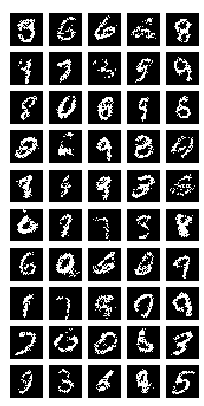
\includegraphics[width=\linewidth]{figs/vae-sample-cropped}
        % 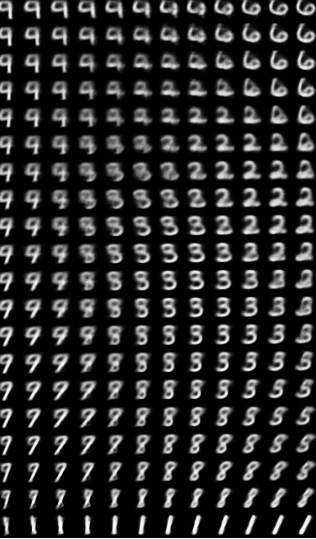
\includegraphics[width=\linewidth]{figs/vae2-cropped}
    \end{columns}
    
    \pause[\thebeamerpauses]
    \alert<.(1)-.(4)>{Note: not a graphical model (desipte shoehorning attempts)}
    \setlength{\fboxsep}{0pt}
    \pause\Put(-300,180){\color{structurecolor}\fbox{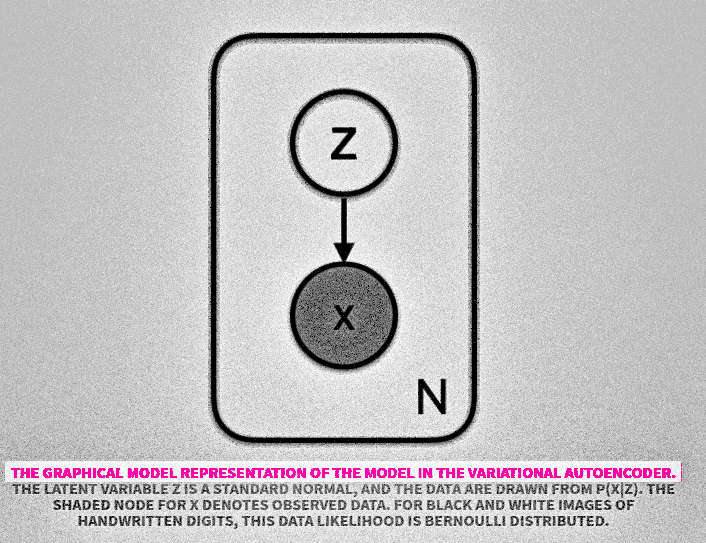
\includegraphics[height=5cm]{figs/vae-diagram-2-colored}}}
    \pause\Put(-130,165){\color{structurecolor}\fbox{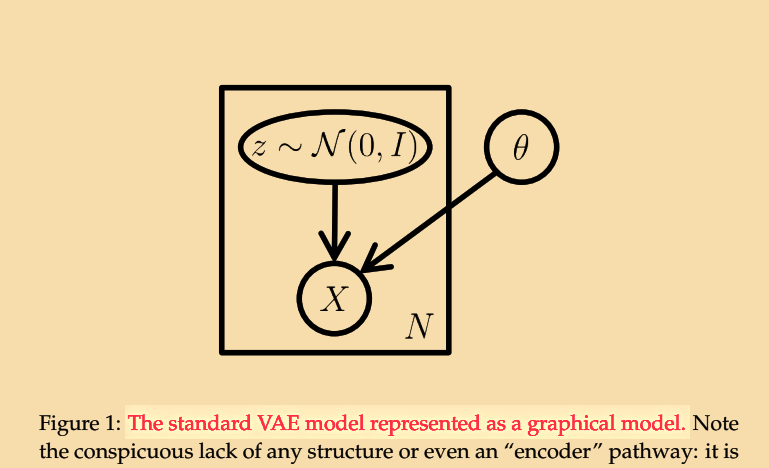
\includegraphics[height=4cm]{figs/vae-diagram-3-colored}}}
    \pause\Put(-200,155){\color{structurecolor}\fbox{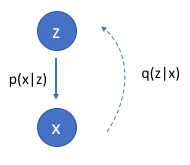
\includegraphics[height=3cm]{figs/vae-diagram-1-cropped}}}
    \pause
    % \Put(10,0){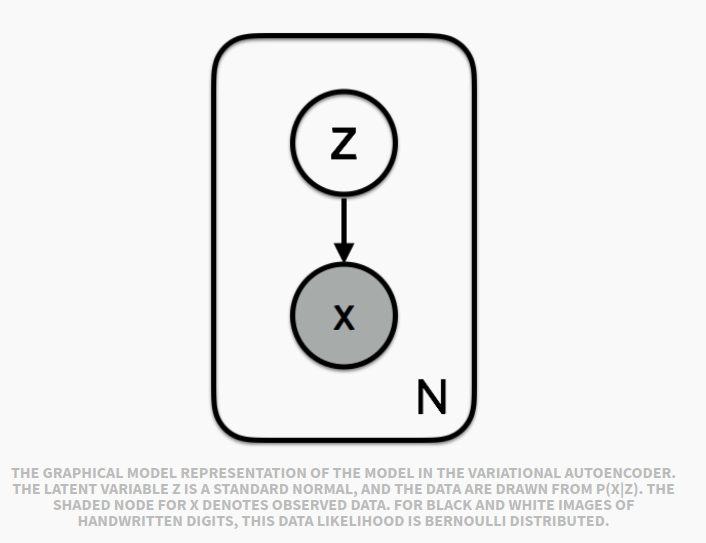
\includegraphics[height=3cm]{figs/vae-diagram-2}}
    \begin{itemize}[<+-|alert@+>]
        \item $e(Z\mid X)$ has same target as $p(Z)$, so BN doesn't work
        \item The heart of the VaE is not its structure, but its objective.
    \end{itemize}
\end{frame}

\begin{frame}
    \frametitle{Variational Auto-Encoders, Take 2}
    
    \begin{itemize}[<+-|alert@+>]
        \item Structure:
        \begin{description}
            % \item generate samples of $X$ from a (smaller) latent space $Z$:     
            \item[$e(Z\mid X)$]: encodes $X$ in a latent space $Z$;
            \item[$d(X\mid Z)$]: generate samples of $X$ from $Z$.
            \item[$p(Z)$]: a prior over from $Z$.
        \end{description}
        \item want to do a gradient step for a specific $x$.
    \end{itemize}
    
		\bigskip
		\onslide<6->{
    \alert<6>{Objective function is free:}}
    \[
        \aar*{\begin{tikzpicture}[center base]
            \node[dpad0] (Z) {$Z$};
            \node[dpad0,right=.5 of Z] (X) {$X$};
            \onslide<2->{
                \draw[arr2, ->, onslide=<2>{alertcolor}] (X) to[bend left=50]
                    node[below]{$e\onslide<5->{\alert<5>{!}}$} (Z); }
            \onslide<3->{
                \draw[arr2, ->, onslide=<3>{alertcolor}] (Z) to[bend left=50]
                    node[above]{$d$} (X); }
            \onslide<5->{
                \draw[arr2, <<-, onslide=<5>{alertcolor}] (X) --
                    node[above,pos=0.8]{$x$}
                    ++(0.9, 0);}
            \onslide<4->{
                \draw[arr2, <-, onslide=<4>{alertcolor}] (Z) --
                    node[above,pos=0.6]{$p$}
                    ++(-0.9, 0);}
        \end{tikzpicture}}
				\alert<6>{\;= \mathrm{ELBO}_{p,e,d}(x)}
    \]
    
\end{frame}

\begin{frame}[label=monotone-inc]
    \frametitle{A Very Useful Fact}
    {\centering Believing more things can't make you any less inconsistent. \par }
    
    \bigskip
    
    {\setbeamercolor{block body}{bg=Emerald!60!gray!20!white}
	 \setbeamercolor{block title}{bg=Emerald!50!structurecolor!35!white}
    \begin{lemma}[monotonicity of inconsistency]\label{lemma!}
     	For all pdgs $\dg M$, $\dg M'$, and all $\gamma > 0$,
    	\begin{enumerate}
    		\item  $\aar{\dg M \sqcup \dg M'}_\gamma \ge \aar{\dg M}_\gamma$.
    		\item If $\dg M$ and $\dg M'$ have respective confidence vectors $\beta$ and $\beta'$, and $\beta \succeq \beta'$ {\color{gray!55}(that is, $\beta_L \ge \beta'_L$ for all $L \in \Ed$)}, then $\aar{\dg M}_\gamma \ge \aar{\dg M'}_\gamma$.
    	\end{enumerate}
    \end{lemma}}
\end{frame}

\begin{frame} %% Visual proof: VaE Variational Bound
    \frametitle{Visual Proof: The Varitaional Bound}
    \begin{align*}
    	\onslide<3->{- \log \Pr\nolimits_{p,d}(X\!=\!x) ~=\hspace{0.8in}&\\[-1.3em]
    	\aar*{\begin{tikzpicture}[center base]
    	   \node[dpad0] (Z) {$Z$};
    	   \node[dpad0,right=.6 of Z] (X) {$X$};
    	   \draw[arr2, ->] (Z) to[bend left=20]
    		   node[above]{$\scriptstyle d$} (X);
    	   \draw[arr2, <<-] (X) --
    		   node[above,pos=0.8]{$\scriptstyle x$}
    		   ++(0.9, 0);
    	   \draw[arr2, <-] (Z) --
    		   node[above,pos=0.6]{$\scriptstyle p$}
    		   ++(-0.9, 0);%
    	\end{tikzpicture}}}
     	&{\onslide<4->{\color{Emerald!50!black}~\le~}}
			\onslide<2->{
	     	\aar*{\begin{tikzpicture}[center base]
	    		\node[dpad0] (Z) {$Z$};
	    		\node[dpad0,right=.5 of Z] (X) {$X$};
	    		\draw[arr2, ->] (X) to[bend left=50]
	    			node[below]{$\scriptstyle e!$} (Z);
	    		\draw[arr2, ->] (Z) to[bend left=50]
	    			node[above]{$\scriptstyle d$} (X);
	    		\draw[arr2, <<-] (X) --
	    			node[above,pos=0.8]{$\scriptstyle x$}
	    			++(0.9, 0);
	    		\draw[arr2, <-] (Z) --
	    			node[above,pos=0.6]{$\scriptstyle p$}
	    			++(-0.9, 0);%
	    	\end{tikzpicture}}
        \\[-0.7em]&\hspace{1.2in}=~ -\mathrm{ELBO}_{p,e,d}(x).}
    \end{align*}
\end{frame}



\subsection{Inconsistency and Statistical Divergences}


\begin{frame}
	\frametitle{Divergences and Inconsistency}
    \begin{lemma}[Divergences and PDGs]
    	The PDG divergence $\thickD^{\mathrm{PDG}}_{(r,s)}(p, q)$, the inconsistency of a PDG containing $p(X)$ with confidence $r$ and $q(X)$ with confidence $s$, is given by
        \[
    		\thickD^{\mathrm{PDG}}_{(r,s)}(p, q) :=
            \aar[\bigg]{\begin{tikzpicture}[center base]
                \node[dpad0] (X) {$X$};
                \draw[arr2, <-] (X) --
    			 		% node[above] {$\overset{(\beta : r)}p$}
    			 		node[above, pos=0.6, inner sep=2pt, align=center] {$p$}
    			 		node[below, pos=0.65, inner sep=3pt, align=center] {$\scriptstyle{\color{gray}(\beta : r)}$}
    				++(-1.1,0);
                \draw[arr2, <-] (X) --
    					% node[above,pos=0.5] {$\overset{(\beta : s)}q$}
    			 		node[above, pos=0.6, inner sep=2pt, align=center] {$q$}
    			 		node[below, pos=0.65, inner sep=3pt, align=center] {$\scriptstyle{\color{gray}(\beta : s)}$}
    				 ++(1.1, 0);
            \end{tikzpicture}}
            % = \thickD^{\mathrm{PDG}}_{(r,s)}(p, q)
            = - (r+s) \log  \sum_x \left(p(x)^{r}\vphantom{\Big|} q(x)^{s}\right)^{\frac{1}{r+s}}.
            % = - (r+s) \log \sum_x \! \sqrt[\leftroot{0}\uproot{2}r+s]{\vphantom{\big|}p(x)^{r} q(x)^{s}}
        % \qquad\text{where}\qquad \xi:= \beta_p+\beta_q
        \]
    \end{lemma}
\end{frame}

\begin{frame}[t] %% Visual Proof: DPI
    \frametitle{Visual Proof: Data Processing Inequality}
		%
		% "light gray script script"
		\def\lgss{\color{gray!80}\scriptscriptstyle}%
		\tikzset{ci2/.style={inner sep=2pt, align=center}}%
		%
		\colorlet{pcolor}{Plum}%
		\colorlet{qcolor}{MidnightBlue}%
		\def\amt{45}%
		\tikzset{pstyle/.style={line width=0.9pt, pcolor!\amt!black}}%
		\tikzset{qstyle/.style={line width=1.3pt, qcolor!\amt!black}}%
		\tikzset{pqstyle/.style={line width=1.5pt,pcolor!50!qcolor!\amt!black}}%
		%
		\def\plabel{{$\lgss\color{pcolor!40}({\beta})$}}
		\def\qlabel{{$\lgss\color{qcolor!40}({\zeta})$}}
		\def\pdgdiv{\thickD^{\mathrm{PDG}}_{\lgss({\color{pcolor!40}\beta},{\color{qcolor!40}\zeta})}\infdivx[\Big]}
		%
		{\color{structurecolor}
			\[ \pdgdiv pq \ge \pdgdiv {f\circ p}{f \circ q}\]}%
		%
    \begin{align*}%
    	% - \log \Pr\nolimits_{p,d}(X\!=\!x) ~=\qquad&\\
    	\aar*{\begin{tikzpicture}[center base]
    	   \node[dpad0] (X) {$X$};
    	   \draw[arr2, <-,qstyle] (X) --
	  		  node[above,pos=0.6,ci2]{$\scriptstyle q$}
					 % node[above,pos=0.6]{$q^{{\color{gray}(s)}}$}
					node[below, pos=0.65,ci2] {\qlabel}
    		   ++(1.1, 0);
    	   \draw[arr2, <-,pstyle] (X) --
				 	node[above,pos=0.6,ci2]{$\scriptstyle p$}
    		   % node[above,pos=0.6]{$p^{{\color{gray}(r)}}$}
					node[below, pos=0.65, ci2] {\plabel}
    		   ++(-1.1, 0);%
    	\end{tikzpicture}}
        &\onslide<2->{= 
        \aar**{\begin{tikzpicture}[center base]
           \node[dpad0] (X) {$X$};
           \node[dpad0,above=.8 of X,align=center] (Y) {$Y$};
           \draw[arr2, <-,qstyle] (X) --
	            node[above,pos=0.6,ci2]{$\scriptstyle q$}
							node[below, pos=0.65,ci2] {\qlabel}
               ++(1.1, 0);
           \draw[arr2, <-,pstyle] (X) --
              node[above,pos=0.6,ci2]{$\scriptstyle p$}
							node[below, pos=0.65,ci2] {\plabel}
               ++(-1.1, 0);%
           \draw[arr2, pqstyle] (X) --
              node[left,pos=0.45,ci2]{$\scriptstyle f$}
							node[right, pos=0.45, inner sep=1pt, align=center] % below,rotate=90
							 	{{$\lgss\color{pcolor!50!qcolor!40}(\beta+\zeta)$}}
              (Y);%
        \end{tikzpicture}}} \\
        &\onslide<3->{= 
        \aar**{\begin{tikzpicture}[center base]
           \node[dpad0] (X1) {$X_1$};
           \node[dpad0, right=0.7 of X1] (X2) {$X_2$};
           \node[dpad0,above=.8 of {$(X1)!.5!(X2)$},align=center] (Y) {$Y$};
           \draw[arr2, -, double equal sign distance] (X1) to (X2);
           \draw[arr2, <-,qstyle] (X2) --
              node[above,pos=0.6,ci2]{$\scriptstyle q$}
							node[below, pos=0.65,ci2] {\qlabel}
              ++(1.1, 0);
           \draw[arr2, <-,pstyle] (X1) --
              node[above,pos=0.6,ci2]{$\scriptstyle p$}
							node[below, pos=0.65,ci2] {\plabel}
              ++(-1.1, 0);%
           \draw[arr2,pstyle] (X1) to[bend left=40]
              node[above left, pos=0.35, inner sep=1pt]{$\scriptstyle f$}
							node[below right=0 and 0, pos=0.45, inner sep=0pt, align=center] {\plabel}
               (Y);%
           \draw[arr2,qstyle] (X2) to[bend right=40]
              node[above right, pos=0.35, inner sep=1pt]{$\scriptstyle f$}
							node[below left=0 and 0, pos=0.45, inner sep=0pt, align=center] {\qlabel}
               (Y);%
        \end{tikzpicture}}}
        \\&\onslide<4->{\ge 
					\aar**{\begin{tikzpicture}[center base]
	           \node[dpad0] (X1) {$X_1$};
	           \node[dpad0, right=0.85 of X1] (X2) {$X_2$};
	           \node[dpad0,above=.65 of {$(X1)!.5!(X2)$},align=center] (Y) {$Y$};
	           \draw[arr2, <-,qstyle] (X2) --
	              node[above,pos=0.6,ci2]{$\scriptstyle q$}
								node[below, pos=0.65,ci2] {\qlabel}
	              ++(1.1, 0);
	           \draw[arr2, <-,pstyle] (X1) --
	              node[above,pos=0.6,pstyle,ci2]{$\scriptstyle p$}
								node[below, pos=0.65,ci2] {\plabel}
	              ++(-1.1, 0);%
	           \draw[arr2,pstyle] (X1) to[bend left=30]
	              node[above left, pos=0.35, inner sep=1pt]{$\scriptstyle f$}
								node[below right=0 and 0, pos=0.45, inner sep=0pt, align=center] {\plabel}
	               (Y);%
	           \draw[arr2,qstyle] (X2) to[bend right=30]
	              node[above right, pos=0.35, inner sep=1pt]{$\scriptstyle f$}
								node[below left=0 and 0, pos=0.45, inner sep=0pt, align=center] {\qlabel}
	               (Y);%
	        \end{tikzpicture}}
        =}
        \aar*{\begin{tikzpicture}[center base]
    	   \node[dpad0] (X) {$X$};
    	   \draw[arr2, <-,qstyle] (X) --
    		   node[above,pos=0.6,ci2]{$\scriptstyle f\circ q$}
					 node[below, pos=0.65,ci2] {\qlabel}
    		   ++(1.1, 0);
    	   \draw[arr2, <-,pstyle] (X) --
    		   node[above,pos=0.6,ci2]{$\scriptstyle f\circ p$}
					 node[below, pos=0.65,ci2] {\plabel}
    		   ++(-1.1, 0);%
    	\end{tikzpicture}}
    \end{align*}
\end{frame}
\begin{frame}\frametitle{Divergences as Inconsistencies}
    \hspace*{-\beamerleftmargin}%
    \resizebox{\paperwidth}{!}{
    	\centering
    	\def\ptradius{0.07}
    	\begin{tikzpicture}[scale=1.8]
    		\draw[help lines, color=gray!30, dashed] (-0.9,-1.4) grid (5.9,2.9);
    		\draw[->,thick] (-1,0)--(6,0) node[right]{$\beta_p$};
    		\draw[->,thick] (0,-1.5)--(0,3) node[above]{$\beta_q$} ;


    		%concave part
    		\fill[gray, fill opacity=0.2] (-1,1) -- (1.5,-1.5) -- (-1,-1.5) --cycle;
    		\draw[gray, opacity=0.5, thick] (-1,1) --
    		node[below left=3em, anchor=north, rotate=-45,font=\footnotesize,fill=gray!20,fill opacity=0.8, inner sep=1pt, outer sep=3pt] % at (-0.5,-0.5)
    			{Non-convex region} (1.5,-1.5);
    		%axis of symmetry
    		% \draw[color=orange!25, thick] (-1, -1) -- (3,3);
    		% \fill[orange, opacity=0.05] (-1,-1) -- (3,3) -- (-1,3) -- cycle;
    		\draw[color=gray!80!orange!45, densely dashdotted] (-1, -1) -- (3,3);
    		\draw[color=gray!80!orange!45, thick, <->] (2.8, 2.2) -- node[above right, anchor=south, rotate=-45,font=\footnotesize,fill=white,fill opacity=0.8, inner sep=1pt, outer sep=3pt]{Axis of Symmtry}(2.2,2.8);


    		% Renyi Entropy Line
    		\draw[blue!40, densely dashed, very thick, opacity=0.8]
    		 	(0,1) -- node[below, align=center, pos=0.8, font=\footnotesize]{R\'enyi divergences\\for $\alpha \in (0,1)$} (5.6,1)
    			(5.6,-1) -- node[above, align=center, pos=0.2, font=\footnotesize]{(negative) R\'enyi divergences\\ for $\alpha \in (1,\infty)$} (1,-1);
    		%Chernoff Information Line
    		\draw[red!40, densely dashed, very thick, opacity=0.9, (-), shorten <=6pt, shorten >=6pt]
    		 	(0,1) -- node[pos=0.5,below left=1ex,anchor=north, rotate=-45, font=\footnotesize, align=center, fill=white,fill opacity=0.8, inner sep=1pt, outer sep=2pt]{Chernoff}
                node[pos=0.5,below left=1.35em, anchor=north, rotate=-45, font=\footnotesize, align=center, fill=white,fill opacity=0.8, inner sep=0.5pt, outer sep=1pt]{Divergences} (1,0);
    		%alpha divergence line
    		\draw[domain=1.5:5.6, smooth, very thick, variable=\x, blue!50!green!50, opacity=0.8, densely dashed] plot ({\x}, {1/(1-1/\x)})
    			node[rotate=-7, font=\footnotesize] at (3.9,1.55){$\alpha$-divergences};

    		%%%% POINTS %%%%
    		%[draw, very thick,fill=magenta!50!black]
    		\fill (0.5,0.5) circle (\ptradius) node[above right, align=center,
    			label={[yshift=0ex,xshift=-1ex,align=left,font=\footnotesize\color{gray!50}]right:Bhattacharya\\distance}]
    			% {Bhattacharya\\distance};
    			% {$\thickD^{\text{Bhattacharya}}$};
    			{$\thickD_{B}(p,q)$};

    		\fill (1,3.4) -- +(0:\ptradius) arc (0:-180:\ptradius) -- +(0:\ptradius)
    			node[below]{$\vdots$}
    			node[right=1ex, align=center,label={[yshift=1ex,xshift=0ex]below:\footnotesize\color{gray!50}Reverse KL}](revKL){$\kldiv qp$};

    		\fill (6.4,1) -- +(270:\ptradius) arc (270:90:\ptradius) -- +(270:\ptradius)
    			node[above=2pt, align=center,
    				label={[yshift=-1ex,xshift=0ex]\footnotesize\color{gray!50} KL Divergence}] (FwdKL) {$\kldiv pq$}
    			node[left]{$\cdots$};

    		\fill (0,1) -- ++(-90:\ptradius) arc (-90:90:\ptradius)
    			node[above right, align=center,
    				label={[yshift=-1ex,xshift=1ex]\footnotesize\color{gray!50} Max Entropy}
    			]{$\I_q(p > 0)$};

    		% divergences requiring negative \beta
    		\fill (2,-1) circle (\ptradius) node[below right, align=center,
    				label={[yshift=1ex,xshift=1ex]below:\footnotesize\color{gray!50}$-\chi^2$ divergence}]
    			{$-\chi^2\infdivx pq$};
    		\fill (1,-1) -- ++(-45:\ptradius) arc (-45:135:\ptradius)
    			node[above, align=center,
    				label={[yshift=-1ex,xshift=1ex]\footnotesize\color{gray!50} $-$Min Entropy}]
    			{$- \log \sup \frac pq$};



    	\end{tikzpicture}
        }
    	% \caption{A map of the inconsistency of the PDG containing the distributions $p(X)$ and $q(X)$, as we vary their respective confidences $\beta_p$ and $\beta_q$. Solid circles indicate well-known named measures, and semicircles indicate limiting values. }
    	% {A map of inconsistency
    	% \(\aar[\bigg]{\begin{tikzpicture}[center base]
    	% 	\node[dpad0] (X) {$X$};
    	% 	\draw[arr2, <-] (X) --
    	% 			node[above, pos=0.6, inner sep=2pt, align=center] {$p$}
    	% 			node[below, pos=0.65, inner sep=3pt, align=center] {$\scriptstyle{\color{gray}(\beta_p)}$}
    	% 		++(-1.1,0);
    	% 	\draw[arr2, <-] (X) --
    	% 			node[above, pos=0.6, inner sep=2pt, align=center] {$q$}
    	% 			node[below, pos=0.65, inner sep=3pt, align=center] {$\scriptstyle{\color{gray}(\beta_q)}$}
    	% 		 ++(1.1, 0);
    	% \end{tikzpicture}}\)
    	% as we vary the confidences $(\beta_p, \beta_q)$ in the distributions $p$ and $q$. }
    	% \label{fig:statdistmap}
        
\end{frame}


\section{Databases}
\begin{frame}
	\TODO[Schema Picture]
	\TODO[Add Universal Relation Theorem]
\end{frame}

\section{Open Problems}
\begin{frame}\frametitle{Open Problems and Future Work}
	\TODO
    % \begin{itemize}
		% 		\item 
    %     \begin{itemize}    
    %         \item Trace Semantics
    %         \item Composition
    %     \end{itemize}
    % \end{itemize}
		
		
\end{frame}

\begin{frame} % Summary
	\frametitle{Summary}
	\TODO[update with second half]
	PDGs\textellipsis 
	\begin{itemize}[<+-|alert@+>]
		\item capture inconsistency, including conflicting information
		from multiple sources with varying reliability.
		\item
			are especially modular; to combine info from two sources, simply take a PDG union.
			This incorporates new data (edge cpds) and concepts (nodes) without affecting previous information.
		\item cleanly separate quantitative info (the cpds) 
			from qualitative info (the edges), with variable confidence
			in both (the weights $\beta$ and $\alpha$).
			This is captured by terms $\Inc$ and $\IDef{}$ in our scoring function.
		\item have (several) natural semantics; one of them allows us to
			pick out a unique distribution.  Using this distrbution, PDGs
			can capture BNs and factor graphs.
			% In the latter case, a simple parameter shift in the corresponding PDG eliminates
			% arguably problematic behavior of a factor graph.
		\end{itemize}
	
	\pause[\thebeamerpauses]
	\medskip
	\textit{But there is much more to be done!}
	\end{frame}
	

\begin{frame}
	\TODO[return to initial slide, but with more conflicts]
\end{frame}


\appendix


\section{Hyper-graphs}
	\colorlet{hypergraphcolor}{benchcolor1}
	\colorlet{simplegraphcolor}{structurecolor}
% \setbeamercolor{background canvas}{bg=black}
%  \setbeamercolor{normal text}{fg=white}
%  \usebeamercolor[fg]{normal text}
 
\begin{frame}[label=hypergraphextra] %%%%%         HYPER-GRAPHS AND GRAPHS      %%%%%%
	\frametitle{{\color{hypergraphcolor}Hyper-graphs?} Or merely {\color{simplegraphcolor!85}graphs}?}
	
	\hfill
	\begin{tikzpicture||precompiled}[center base,draw=hypergraphcolor]{grok-pre}
		\fill[fill opacity=0.07,hypergraphcolor, draw, draw opacity=0.2]
			(-0.6,0.6) rectangle (2.1, -2.1);

		\node[dpadded] (C) at (0,0) {$\mathit C$};
		\node[dpadded] (T) at (1.5,0){$\mathit T$};
		\node[dpadded] (SL) at (.75,-1.5){$\it SL$};

		\draw[arr] (T) to[bend right]  (C);
		\alert<2>{ \mergearr{C}{T}{SL} }
		% \drawbb
		\end{tikzpicture||precompiled}
	\onslide<2->{
		\hfill
		\begin{tikzpicture||precompiled}[center base]{widget}%[center base]
		\fill[fill opacity=0.07,simplegraphcolor, draw, draw opacity=0.2]
			(-2.1,-1.85) rectangle (2.1, 1.6);

			\node[dpadded] (SL) at (0,-1.3) {$\mathit{SL}$};

			\node[dpadded] (C) at (-1.5,1) {$\mathit C$};
			\node[dpadded] (T) at (1.5,1) {$\mathit T$};

			\alert<2>{
				\node[dpadded,light pad] (CT) at (0, 0){$\scriptstyle C \times T$};
				\draw[arr1, ->>] (CT) -- (C);
				\draw[arr1, ->>] (CT) -- (T);
				\draw[arr1] (CT) -- (SL);
				}
			\draw[arr] (T) to [bend right=15] (C);
			% \drawbb
			\end{tikzpicture||precompiled}
		}
		\hfill~
	\onslide<3->{
		\vspace{1em}
		\begin{itemize}
			\item<3-|alert@+> This widget expands state space, but graphs are simpler.
			\item<4-> \alert<4>{There is a natural correspondence}
			\[ \text{\color{hypergraphcolor} joint distributions}\quad\leftrightarrows\quad\parbox{15em}{\color{simplegraphcolor}\centering expanded joint distributions\\ satisfying coherence constraints} \]
		\end{itemize}
		}
	\onslide<5->
		{\small\color{gray} (working directly with hypergraphs is also possible)}
	
	\vskip0pt plus 1filll
	\hfill\hyperlink{definition}{\beamerbutton{main definition}}
	\end{frame} %----------

\begin{frame}[label=idefextra]\frametitle{Illustrations of $\IDef{}$}
	\def\vsize{0.4}
	\vskip0pt plus 1filll
	% \tikzset{dpad0/.append style={fill opacity=0.1}}
	\begin{tikzpicture}[center base,scale=1.5] %\label{subfig:justXY}
		% \node[dpad0] (1) at (0,2){$\pdgunit$};
		\node[dpad0] (X) at (-0.45,.85){$X$};
		\node[dpad0] (Y) at (0.45,.85){$Y$};
		\path[fill=green!50!black] (-0.2,0) circle (\vsize) ++(-110:.26) node[label=below:\tiny$X$]{};
		\path[fill=green!50!black] (0.2,0) circle (\vsize) ++(-70:.26) node[label=below:\tiny$Y$]{};
		\begin{scope}
			\clip (-0.2,0) circle (\vsize);
			\clip (0.2,0) circle (\vsize);
			\fill[green!50!black] (-1,-1) rectangle (3,3);
			% \draw[ultra thick,white] (-0.2,0) circle (\vsize);
			% \draw[ultra thick,white] (0.2,0) circle (\vsize);
		\end{scope}
		\draw (-0.2,0) circle (\vsize);
		\draw (0.2,0) circle (\vsize);
		\useasboundingbox (current bounding box);
		\node at (-0.8, 0.4){};
		\end{tikzpicture}$\qquad$
	%% EXAMPLE: X -> Y
	\begin{tikzpicture}[center base,scale=1.5]%\label{subfig:XtoY}
		% \node[dpad0] (1) at (0,2){$\pdgunit$};
		\node[dpad0] (X) at (-0.45,0.85){$X$};
		\node[dpad0] (Y) at (0.45,0.85){$Y$};
		\draw[arr] (X) to[] (Y);
		% \draw[arr] (1) to[] (Y);
		\path[fill=green!50!black] (-0.2,0) circle (\vsize) ++(-110:.26) node[label=below:\tiny$X$]{};
		\path[fill=white!70!black] (0.2,0) circle (\vsize) ++(-70:.26) node[label=below:\tiny$Y$]{};
		\begin{scope}
			\clip (-0.2,0) circle (\vsize);
			\clip (0.2,0) circle (\vsize);
			\fill[green!50!black] (-1,-1) rectangle (3,3);
			% \draw[ultra thick,white] (-0.2,0) circle (\vsize);
			% \draw[ultra thick,white] (0.2,0) circle (\vsize);
		\end{scope}
		\draw (-0.2,0) circle (\vsize);
		\draw (0.2,0) circle (\vsize);
		\useasboundingbox (current bounding box);
		\node at (-0.8, 0.4){};
		\end{tikzpicture}$\qquad$		
	%% EXAMPLE: X ->> Y
	\begin{tikzpicture}[center base,scale=1.5]%\label{subfig:XtoY}
		% \node[dpad0] (1) at (0,2){$\pdgunit$};
		\node[dpad0] (X) at (-0.45,0.85){$X$};
		\node[dpad0] (Y) at (0.45,0.85){$Y$};
		\draw[arr,->>] (X) to[] (Y);
		% \draw[arr] (1) to[] (Y);
		\path[fill=green!50!black] (-0.2,0) circle (\vsize) ++(-110:.26) node[label=below:\tiny$X$]{};
		\path[fill=red!50!black] (0.2,0) circle (\vsize) ++(-70:.26) node[label=below:\tiny$Y$]{};
		\begin{scope}
			\clip (-0.2,0) circle (\vsize);
			\clip (0.2,0) circle (\vsize);
			\fill[green!50!black] (-1,-1) rectangle (3,3);
			% \draw[ultra thick,white] (-0.2,0) circle (\vsize);
			% \draw[ultra thick,white] (0.2,0) circle (\vsize);
		\end{scope}
		\draw (-0.2,0) circle (\vsize);
		\draw (0.2,0) circle (\vsize);
		\useasboundingbox (current bounding box);
		\node at (-0.8, 0.4){};
		\end{tikzpicture}$\qquad$		
	%% EXAMPLE: X <-> Y
	\begin{tikzpicture}[center base,scale=1.5] %\label{subfig:XY-cycle}
		% \node[dpad0] (1) at (0,2){$\pdgunit$};
		\node[dpad0] (X) at (-0.45,0.85){$X$};
		\node[dpad0] (Y) at (0.45,0.85){$Y$};
		\draw[arr] (X) to[bend left] (Y);
		\draw[arr] (Y) to[bend left] (X);
		\draw[fill=white!70!black] (-0.2,0) circle (\vsize) ++(-110:.26) node[label=below:\tiny$X$]{};
		\draw[fill=white!70!black] (0.2,0) circle (\vsize) ++(-70:.26) node[label=below:\tiny$Y$]{};
		\begin{scope}
			\clip (-0.2,0) circle (\vsize);
			\clip (0.2,0) circle (\vsize);
			\fill[green!50!black] (-1,-1) rectangle (3,3);
			% \draw[ultra thick,white] (-0.2,0) circle (\vsize);
			% \draw[ultra thick,white] (0.2,0) circle (\vsize);
		\end{scope}
		\draw (-0.2,0) circle (\vsize);
		\draw (0.2,0) circle (\vsize);
		\useasboundingbox (current bounding box.south west) rectangle (current bounding box.north east);
		\node at (-0.85, 0.4){};
		\end{tikzpicture}
		
		\vskip0pt plus 1filll
		\hfill
		% \hyperlink{returntosemantics}{\beamerbutton{back to semantics}}
	\end{frame}
\begin{frame}
	\def\vsize{0.4}
	\def\bnslide{4}
	\def\spacerlength{0.5em}
	\begin{tikzpicture}[center base]\label{subfig:justX-0}
		\node[dpad0] (X) at (0,1){$X$};
		\draw[fill=green!50!black]  (0,0) circle (\vsize)  ++(-90:.22) node[label=below:\tiny$X$]{};
		\useasboundingbox (current bounding box);
		\node at (-0.5, 0.6){};
		\end{tikzpicture}
	\begin{tabular}{c}
	\begin{tikzpicture}[onslide=<\bnslide>{is bn}]\label{subfig:justX-1}
		\node[dpad0] (1) at (-0.4,.85){$\!\pdgunit\!$};
		\node[dpad0] (X) at (0.4,.85){$X$};
		\draw[arr1] (1)  -- (X);
		\draw[fill=white!70!black]  (0,0) circle (\vsize) ++(-90:.22) node[label=below:\tiny$X$]{};
		\node at (-0.6,0.35){};
		\useasboundingbox (current bounding box);
		\node at (-0.7, 0.35){};
		\end{tikzpicture} \\[0.5em]
	\begin{tikzpicture}\label{subfig:justX-2}
		\node[dpad0] (1) at  (-0.45,.85){$\!\pdgunit\!$};
		\node[dpad0] (X) at  (0.45,.85){$X$};
		\draw[arr1] (1) to[bend left=20] (X);
		\draw[arr1] (1) to[bend right=20] (X);
		\draw[fill=red!50!black] (0,0) circle (\vsize) ++(-90:.22) node[label=below:\tiny$X$]{};
		\useasboundingbox (current bounding box);
		\node at (-0.7, 0.35){};
		\end{tikzpicture}
	\end{tabular}%}
	\hspace{\spacerlength}\vrule\hspace{\spacerlength}
	%% EXAMPLE: X  Y
	% \adjustbox{valign=b}{
	\begin{tabular}{c}
	\begin{tikzpicture}[]  \label{subfig:justXY}
		% \node[dpad0] (1) at (0,2){$\pdgunit$};
		\node[dpad0] (X) at (-0.45,.85){$X$};
		\node[dpad0] (Y) at (0.45,.85){$Y$};
		\path[fill=green!50!black] (-0.2,0) circle (\vsize) ++(-110:.23) node[label=below:\tiny$X$]{};
		\path[fill=green!50!black] (0.2,0) circle (\vsize) ++(-70:.23) node[label=below:\tiny$Y$]{};
		\begin{scope}
			\clip (-0.2,0) circle (\vsize);
			\clip (0.2,0) circle (\vsize);
			\fill[green!50!black] (-1,-1) rectangle (3,3);
			% \draw[ultra thick,white] (-0.2,0) circle (\vsize);
			% \draw[ultra thick,white] (0.2,0) circle (\vsize);
		\end{scope}
		\draw (-0.2,0) circle (\vsize);
		\draw (0.2,0) circle (\vsize);
		\useasboundingbox (current bounding box);
		\node at (-0.8, 0.4){};
		\end{tikzpicture}\\[0.5em]
	%% EXAMPLE: X -> Y
	\begin{tikzpicture}[]\label{subfig:XtoY}
		% \node[dpad0] (1) at (0,2){$\pdgunit$};
		\node[dpad0] (X) at (-0.45,0.85){$X$};
		\node[dpad0] (Y) at (0.45,0.85){$Y$};
		\draw[arr1] (X) to[] (Y);
		% \draw[arr] (1) to[] (Y);
		\path[fill=green!50!black] (-0.2,0) circle (\vsize) ++(-110:.23) node[label=below:\tiny$X$]{};
		\path[fill=white!70!black] (0.2,0) circle (\vsize) ++(-70:.23) node[label=below:\tiny$Y$]{};
		\begin{scope}
			\clip (-0.2,0) circle (\vsize);
			\clip (0.2,0) circle (\vsize);
			\fill[green!50!black] (-1,-1) rectangle (3,3);
			% \draw[ultra thick,white] (-0.2,0) circle (\vsize);
			% \draw[ultra thick,white] (0.2,0) circle (\vsize);
		\end{scope}
		\draw (-0.2,0) circle (\vsize);
		\draw (0.2,0) circle (\vsize);
		\useasboundingbox (current bounding box);
		\node at (-0.8, 0.4){};
		\end{tikzpicture}
	\end{tabular}%}
	% \hspace{\spacerlength}
	\begin{tabular}{c}
	%% EXAMPLE: X <-> Y
	\begin{tikzpicture}[center base]\label{subfig:XY-cycle}
		% \node[dpad0] (1) at (0,2){$\pdgunit$};
		\node[dpad0] (X) at (-0.45,0.85){$X$};
		\node[dpad0] (Y) at (0.45,0.85){$Y$};
		\draw[arr1] (X) to[bend left] (Y);
		\draw[arr1] (Y) to[bend left] (X);
		\draw[fill=white!70!black] (-0.2,0) circle (\vsize) ++(-110:.25) node[label=below:\tiny$X$]{};
		\draw[fill=white!70!black] (0.2,0) circle (\vsize) ++(-70:.25) node[label=below:\tiny$Y$]{};
		\begin{scope}
			\clip (-0.2,0) circle (\vsize);
			\clip (0.2,0) circle (\vsize);
			\fill[green!50!black] (-1,-1) rectangle (3,3);
			% \draw[ultra thick,white] (-0.2,0) circle (\vsize);
			% \draw[ultra thick,white] (0.2,0) circle (\vsize);
		\end{scope}
		\draw (-0.2,0) circle (\vsize);
		\draw (0.2,0) circle (\vsize);
		\useasboundingbox (current bounding box.south west) rectangle (current bounding box.north east);
		\node at (-0.85, 0.4){};
		\end{tikzpicture}\\[2.5em]
	% \hspace{\spacerlength}%% EXAMPLE: 1 -> Y;1->X
		\begin{tikzpicture}[center base, onslide=<\bnslide>{is bn}] \label{subfig:XYindep}
		\node[dpad0] (1) at (0,0.75){$\!\pdgunit\!$};
		\node[dpad0] (X) at (-0.7,0.95){$X$};
		\node[dpad0] (Y) at (0.7,0.95){$Y$};
		\draw[arr0] (1) to[] (X);
		\draw[arr0] (1) to[] (Y);
		\draw[fill=white!70!black] (-0.2,0) circle (\vsize) ++(-110:.23) node[label=below:\tiny$X$]{};
		\draw[fill=white!70!black] (0.2,0) circle (\vsize) ++(-70:.23) node[label=below:\tiny$Y$]{};
		\begin{scope}
			\clip (-0.2,0) circle (\vsize);
			\clip (0.2,0) circle (\vsize);
			\fill[red!50!black] (-1,-1) rectangle (3,3);
			% \draw[ultra thick,white] (-0.2,0) circle (\vsize);
		% \draw[ultra thick,white] (0.2,0) circle (\vsize);
		\end{scope}
		\draw (-0.2,0) circle (\vsize);
		\draw (0.2,0) circle (\vsize);
		\useasboundingbox (current bounding box.south west) rectangle (current bounding box.north east);
		\node at (-0.88, 0.4){};
		\end{tikzpicture}
	\end{tabular}
	\hspace{\spacerlength}
	 %% EXAMPLE: 1 -> X -> Y
	\begin{tikzpicture}[center base, onslide=<\bnslide>{is bn}]\label{subfig:1XY}
		\node[dpad0] (1) at (0.15,2){$\!\pdgunit\!$};
		\node[dpad0] (X) at (-0.45,1.4){$X$};
		\node[dpad0] (Y) at (0.35,1){$Y$};
		\draw[arr0] (1) to[] (X);
		\draw[arr1] (X) to[] (Y);
		\path[fill=white!70!black] (-0.2,0) circle (\vsize) ++(-110:.23) node[label=below:\tiny$X$]{};
		\path[fill=white!70!black] (0.2,0) circle (\vsize) ++(-70:.23) node[label=below:\tiny$Y$]{};
		\begin{scope}
			\clip (-0.2,0) circle (\vsize);
			\clip (0.2,0) circle (\vsize);
			% \fill[red!50!black] (-1,-1) rectangle (3,3);
			% \draw[ultra thick,white] (-0.2,0) circle (\vsize);
			% \draw[ultra thick,white] (0.2,0) circle (\vsize);					\end{scope}
		\end{scope}
		\draw (-0.2,0) circle (\vsize);
		\draw (0.2,0) circle (\vsize);
		\useasboundingbox (current bounding box);
		\node at (-0.7, 0.6){};
		\end{tikzpicture}
	% \hspace{\spacerlength}\hspace{2.5pt}\vrule\hspace{2.5pt}\hspace{\spacerlength}

	\vspace{0.5em}
	%% EXAMPLE: 1 -> X -> Y -> Z
	\begin{tikzpicture}[center base, onslide=<\bnslide>{is bn}] \label{subfig:1XYZ}
		% \node[dpad0] (1) at (-0.5,2.3){$\!\pdgunit\!$};
		% \node[dpad0] (X) at (-0.5,1.5){$X$};
		% \node[dpad0] (Y) at (0.35,1.25){$Y$};
		% \node[dpad0] (Z) at (0.25,2.25){$Z$};
		\node[dpad0] (1) at (-1,0.8){$\!\pdgunit\!$};
		\node[dpad0] (X) at (-0.6,1.6){$X$};
		\node[dpad0] (Y) at (0.35,1.6){$Y$};
		\node[dpad0] (Z) at (1.0,0.9){$Z$};
		\draw[arr0] (1) to (X);
		\draw[arr1] (X) to[] (Y);
		\draw[arr1] (Y) to[] (Z);
		\path[fill=white!70!black] (210:0.22) circle (\vsize) ++(-130:.25) node[label=below:\tiny$X$]{};
		\path[fill=white!70!black] (-30:0.22) circle (\vsize) ++(-50:.25) node[label=below:\tiny$Y$]{};
		\path[fill=white!70!black] (90:0.22) circle (\vsize) ++(40:.29) node[label=above:\tiny$Z$]{};
		\begin{scope}
			\clip (90:0.22) circle (\vsize);
			\clip (210:0.22) circle (\vsize);
			\fill[red!50!black] (-1,-1) rectangle (3,3);
			% \draw[ultra thick,white] (210:0.2) circle (\vsize);
			% \draw[ultra thick,white] (90:0.2) circle (\vsize);
			\clip (-30:0.22) circle (\vsize);
			\fill[white!70!black] (-1,-1) rectangle (3,3);
			% \draw[ultra thick,white] (-30:0.2) circle (\vsize);
			% \draw[ultra thick,white] (210:0.2) circle (\vsize);
			% \draw[ultra thick,white] (90:0.2) circle (\vsize);
		\end{scope}
		\begin{scope}
			\draw[] (-30:0.22) circle (\vsize);
			\draw[] (210:0.22) circle (\vsize);
			\draw[] (90:0.22) circle (\vsize);
		\end{scope}
		\useasboundingbox (current bounding box);
		\node at (-0.7, 0.7){};
		\end{tikzpicture}
	%% EXAMPLE: X -> Y -> Z -> X
	\hspace{\spacerlength}
	\begin{tikzpicture}[center base] \label{subfig:XYZ-cycle}
		% \node[dpad0] (1) at (-0.5,2.3){$\pdgunit$};
		\node[dpad0] (X) at (-0.5,1.75){$X$};
		\node[dpad0] (Y) at (0.35,1.25){$Y$};
		\node[dpad0] (Z) at (0.25,2.25){$Z$};
		% \draw[arr0] (1) to (X);
		\draw[arr1] (X) to[bend right=25] (Y);
		\draw[arr1] (Y) to[bend right=25] (Z);
		\draw[arr1] (Z) to[bend right=25] (X);
		%option: -- either X -> Y -> Z -> X, or <-> Y <-> Z <-> X. For the latter, uncomment the 6 lines below and comment out the next 3.
		% \draw[arr1] (Z) to[bend left=5] (Y);
		% \draw[arr1] (Y) to[bend left=5] (X);
		% \draw[arr1] (X) to[bend left=5] (Z);
		% \draw[fill=red!50!black] (210:0.22) circle (\vsize) ++(-130:.27) node[label=below:\tiny$X$]{};
		% \draw[fill=red!50!black] (-30:0.22) circle (\vsize) ++(-50:.27) node[label=below:\tiny$Y$]{};
		% \draw[fill=red!50!black] (90:0.22) circle (\vsize) ++(140:.31) node[label=above:\tiny$Z$]{};

		% grey filling for one covering.
		\draw[fill=white!70!black] (210:0.22) circle (\vsize) ++(-130:.27) node[label=below:\tiny$X$]{};
		\draw[fill=white!70!black] (-30:0.22) circle (\vsize) ++(-50:.27) node[label=below:\tiny$Y$]{};
		\draw[fill=white!70!black] (90:0.22) circle (\vsize) ++(40:.31) node[label=above:\tiny$Z$]{};

		\begin{scope}
			\clip (-30:0.22) circle (\vsize);
			\clip (210:0.22) circle (\vsize);
			% \fill[white!70!black] (-1,-1) rectangle (3,3);
			\clip (90:0.22) circle (\vsize);
			\fill[green!50!black] (-1,-1) rectangle (3,3);
		\end{scope}
		\begin{scope}
			\draw[] (-30:0.22) circle (\vsize);
			\draw[] (210:0.22) circle (\vsize);
			\draw[] (90:0.22) circle (\vsize);
		\end{scope}
		\useasboundingbox (current bounding box);
		\node at (-0.7, 0.7){};
		\end{tikzpicture}
	%% EXAMPLE: X -> Y <- Z
	\hspace{\spacerlength}
	\begin{tikzpicture}[center base] \label{subfig:XZtoY}
		% \node[dpad0] (1) at (-0.5,2.3){$\pdgunit$};
		\node[dpad0] (X) at (-0.45,1.9){$X$};
		\node[dpad0] (Y) at (0.3,1.25){$Y$};
		\node[dpad0] (Z) at (0.4,2.15){$Z$};
		% \draw[arr0] (1) to (X);
		\draw[arr0] (X) to[] (Y);
		\draw[arr1] (Z) to[] (Y);
		\path[fill=green!50!black] (210:0.22) circle (\vsize) ++(-130:.25) node[label=below:\tiny$X$]{};
		\path[fill=red!50!black] (-30:0.22) circle (\vsize) ++(-50:.25) node[label=below:\tiny$Y$]{};
		\path[fill=green!50!black] (90:0.22) circle (\vsize) ++(40:.29) node[label=above:\tiny$Z$]{};
		\begin{scope}
			\clip (-30:0.22) circle (\vsize);
			\clip (90:0.22) circle (\vsize);
			\fill[white!70!black] (-1,-1) rectangle (3,3);
		\end{scope}
		\begin{scope}
			\clip (-30:0.22) circle (\vsize);
			\clip (210:0.22) circle (\vsize);
			\fill[white!70!black] (-1,-1) rectangle (3,3);

			\clip (90:0.22) circle (\vsize);
			\fill[green!50!black] (-1,-1) rectangle (3,3);
			% \draw[ultra thick,white] (210:0.2) circle (\vsize);
			% \draw[ultra thick,white] (90:0.2) circle (\vsize);
			% \draw[ultra thick,white] (-30:0.2) circle (\vsize);
			% \draw[ultra thick,white] (210:0.2) circle (\vsize);
			% \draw[ultra thick,white] (90:0.2) circle (\vsize);
		\end{scope}
		\draw[] (-30:0.22) circle (\vsize);
		\draw[] (210:0.22) circle (\vsize);
		\draw[] (90:0.22) circle (\vsize);
		\useasboundingbox (current bounding box);
		% \node at (-0.7, 0.7){};
		\end{tikzpicture}
	%% EXAMPLE: X <-> Y <-> Z
	\hspace{\spacerlength}
	\begin{tikzpicture}[center base] \label{subfig:XYZ-bichain}
		% \node[dpad0] (1) at (0.1,2.4){$\pdgunit$};
		\node[dpad0] (X) at (-1,1.2){$X$};
		\node[dpad0] (Y) at (0,1.7){$Y$};
		\node[dpad0] (Z) at (1,1.4){$Z$};
		% \draw[arr1] (1) to (X);
		% \draw[arr1] (1) to (Y);
		\draw[arr1] (X) to[bend right=15] (Y);
		\draw[arr1] (Y) to[bend right=15] (X);
		\draw[arr1] (Y) to[bend right=15] (Z);
		\draw[arr1] (Z) to[bend right=15] (Y);
		\path[fill=white!70!black] (210:0.22) circle (\vsize) ++(-130:.25) node[label=below:\tiny$X$]{};
		\path[fill=red!50!black] (-30:0.22) circle (\vsize) ++(-50:.25) node[label=below:\tiny$Y$]{};
		\path[fill=white!70!black] (90:0.22) circle (\vsize) ++(40:.29) node[label=above:\tiny$Z$]{};
		\begin{scope}
			\clip (-30:0.22) circle (\vsize);
			\clip (90:0.22) circle (\vsize);
			\fill[white!70!black] (-1,-1) rectangle (3,3);
		\end{scope}
		\begin{scope}
			\clip (90:0.22) circle (\vsize);
			\clip (210:0.22) circle (\vsize);
			\fill[red!50!black] (-1,-1) rectangle (3,3);
		\end{scope}
		\begin{scope}
			\clip (-30:0.22) circle (\vsize);
			\clip (210:0.22) circle (\vsize);
			\fill[white!70!black] (-1,-1) rectangle (3,3);

			\clip (90:0.22) circle (\vsize);
			\fill[green!50!black] (-1,-1) rectangle (3,3);
			% \draw[ultra thick,white] (210:0.2) circle (\vsize);
			% \draw[ultra thick,white] (90:0.2) circle (\vsize);
			% \draw[ultra thick,white] (-30:0.2) circle (\vsize);
			% \draw[ultra thick,white] (210:0.2) circle (\vsize);
			% \draw[ultra thick,white] (90:0.2) circle (\vsize);
		\end{scope}
		\draw[] (-30:0.22) circle (\vsize);
		\draw[] (210:0.22) circle (\vsize);
		\draw[] (90:0.22) circle (\vsize);
		\useasboundingbox (current bounding box);
		\node at (-0.7, 0.7){};
		\end{tikzpicture}
	\end{frame}


\section{Category Theory}
{
    \subsection{PDGs as diagrams of the Markov Category}
    \setbeamercolor{background canvas}{bg=structurecolor!45!gray!25!black}
    \setbeamercolor{normal text}{fg=white!75!black}
    % \setbeamercolor{itemize item}{fg=yellow}
    \setbeamertemplate{itemize item}[circle]
    \begin{frame} %%%%%%%%%%%%% Definition of PDG, details (removed for AAAI) %%%%%%%%%%%
    	% \colorlet{notationcolor}{benchcolor2!40!alertcolor}
    	\setbeamercolor{alerted notation}{fg=benchcolor2!40!alertcolor}
    	\setbeamercolor{base notation}{fg=notationcolor!60!black}
        \setbeamercolor{notation}{use={base notation},fg=base notation.fg}
    	\setbeamercolor{block body}{bg=structurecolor!05!black}
    	\setbeamercolor{block title}
            {bg=structurecolor!40!black,fg=structurecolor!30!white}
        \usebeamercolor{background canvas}
        \usebeamercolor[fg]{normal text}

    	\setlength{\pdgdefnwidth}{0.55\textwidth}
    	% \vspace{-1.5em}
    	\begin{columns}[t]
        % \column{0.5\textwidth-0.5\pdgdefnwidth}
        % \hfill% \dotfill
		\column{\pdgdefnwidth}
		\begin{defn}[PDG]
			\begin{description}%
                \only<6>{\setbeamercolor{alerted text}{fg=benchcolor2}%
                    \setbeamercolor{alerted notation}{fg=benchcolor2!60!gray!50!black}}
                % \color<6>{benchcolor2}
				\item[$\N$]<alert@1-4,6|hideme@5>%<hideme@5|alert@1-4,6>
                    % \notation{\color<6>{benchcolor2!60!gray!50!black}$:\Set$}<1-4,6>%
                    \notation{$:\Set$}%
					\hfill\small (node set)
					\begin{description}
                        \only<6>{\setbeamercolor{alerted text}{fg=benchcolor1}%
                            \setbeamercolor{alerted notation}{fg=benchcolor1!60!gray!50!black}}
                        % \color<6>{benchcolor1}
						\item[$\V$]<hideme@2,3,5|alert@6>
                            % \color<6>{benchcolor1!60!gray!50!black}
                            \notation{$:\N \to \Set$}
                            % \!{\color<1,4>{notationcolor}\color<6>{benchcolor1!60!gray!50!black}{$:\N \to \Set$}}\quad%                         
							\hfill\small (node values)%
						\end{description}

                \only<6>{\setbeamercolor{alerted text}{fg=benchcolor2}%
                    \setbeamercolor{notation}{fg=benchcolor2!60!gray!50!black}}
				\item[$\Ed$]<hideme@1,5 |alert@2-4,6> \notation{\color<6>{benchcolor2!60!gray!50!black}%
                        $\subseteq \N \times \N \times \mathit{Label}$}%<2-4,6>%
                        % $: \Set$}<2->%
					\hfill\small (edge set)\\[0.14em]
					{\color{gray!70!white}For $\ed LXY \in \Ed$,}
					%, each with a source $X$ and target $Y$ in $\N$;
					\begin{description}%[<+-| alert@+>]
                        % \item[$\mathrm{src}$]<hideme@1 |alert@2-6>
                        %     \notation{\color<6>{benchcolor2!50!black}$:\Ed \to \N$}<2->%
                        %     \hfill\small (edge source)%
                        % \item[$\mathrm{tgt}$]<hideme@1 |alert@2-6>
                        %     \notation{\color<6>{benchcolor2!50!black}$:\Ed \to \N$}<2->%
                        %     \hfill\small (edge target)%
                        % \only<6>{\setbeamercolor{alerted text}{fg=benchcolor1}%
                        %     % \usebeamercolor[fg]{alerted text}
                        %     }
                        \only<6>{\setbeamercolor{alerted text}{fg=benchcolor1}%
                            \setbeamercolor{alerted notation}{fg=benchcolor1!60!gray!50!black}}
                        % \color<6>{benchcolor1}
						\item[$\bp$]<hideme@1-3,5 | alert@4,6> %:\big(\!(X,Y,\ell)\in\!\Ed \big) \to
							% \!{\color<4>{notationcolor}\color<6>{benchcolor1!60!gray!50!black}
                                \notation{$:\V(X) \to \Delta\V(Y)$}%
                                % {$:(L:\Ed) \to \V(\mathrm{src} L) \to \Delta\V(\mathrm{tgt} L)$}}%
							\hfill\small (edge cpd)
                        % }
                        % \onslide<-5>{
						\item[$\alpha\ssub L$]<hideme@1-2,4-> \notation{$: \mathbb R$}%
							\hfill\small(functional determination)
						\item[$\beta\ssub L$]<hideme@1-> \notation{$: \mathbb R$}%
							\hfill\small(cpd confidence)
                        % }                        
						\end{description}
				\end{description}
			\end{defn}
			\column{1.0\textwidth-1.0\pdgdefnwidth}
            % \hfill % \dotfill
        	\begin{itemize}
        		% \onslide<1>{\item<1-|alert@+> $(\N, \V) \cong $ \texttt{Set<Variable>}\\[-1em]}
        		\item<1-|alert@+> $(\N, \V)$ is a set of variables % \cong $ \texttt{Set<Variable>}
        		\item<2-|alert@+> $(\N, \Ed)$ is a multigraph % \cong $ \texttt{MultiGraph}
        		\item<3-|alert@+> $(\N, \Ed, \alpha)$, the qualitative data, forms a weighted multigraph.
        		\item<4-> \alert<+>{We call $(\N, \Ed, \V, \mat p)$ an \emph{unweighted} PDG}
        			\begin{itemize}
        					\item {\color{gray} and give it semantics as though $\alpha_L = \beta_L = 1$.}
        					% \item $(\N, \Ed, \V)$ are (mostly) implicit in $\mat p$,
        					% 	and so \\ ``collection of cpds'' $\cong$ \texttt{UnweightedPDG}.
        				\end{itemize}
        		\end{itemize}
		\end{columns}
		
	\vspace{1em}
    \onslide<5->{\alert<5>{
        Let ${\color{white}\mathbf{Mark}}$ be the category of measurable spaces and Markov kernels.}}
    
    % \setbeamercolor{normal text}{fg=black}
    % \usebeamercolor[fg]{normal text}
    \setbeamercolor{block body}{bg=alertcolor!15!black}
	\setbeamercolor{block title}{bg=alertcolor!30!black,fg=alertcolor}
    \setbeamercolor{normal text}{fg=white!75!black}
    \usebeamercolor[fg]{normal text}
	\begin{block}<6>{Equivalent Categorical Definition}
		An unweighted PDG is a functor
		${\color{benchcolor1}\langle \mat p, \V\rangle}\colon {\color{benchcolor2}\mathit{Paths}(\N, \Ed)} \to {\color{white}\mathbf{Mark}}$.
        
        So a PDG is a \emph{diagram} in ${\color{white}\mathbf{Mark}}$, in the usual mathematical sense.
		\end{block}
	\end{frame}
    
    \setbeamercolor{normal text}{fg=white!75!black}
    \begin{frame}
        \usebeamercolor[fg]{normal text}
        What do you do with diagrams? Take {\color{blue!50!gray!60!white}limits} 
        {\color{gray!40!black}/ colimits}.
        
        
        \onslide<+->{
        \begin{center}
            \begin{tikzpicture}[scale=1.2]
                \begin{scope}[every node/.style={outer sep=0pt,inner sep=1pt}]
                    \node (dots-left) at (-2, 0) {$\cdots$};
                    \node (X1) at (-1,0) {$X_1$};
                    \node (X2) at (0,-0.2) {$X_2$};
                    \node (X3) at (1,0) {$X_3$};
                    \node (dots-right) at (2,0) {$\cdots$};
                \end{scope}
                
                \onslide<+(1)->{
                    \begin{scope}[red!30!gray!70!black]
                        \node (V) at (-0.5,1.2){$V$};
                        \draw[arr2] (V) -- (X1);
                        \draw[arr2] (V) -- (X2);
                        \draw[arr2] (V) -- (X3);
                        
                        \node[below left=0.05 and 0.1 of V,inner sep=0pt, outer sep=0pt] {$\scriptstyle\forall$};
                    \end{scope}
                }
                
                \onslide<+(-1)->{
                    \begin{scope}[blue!50!gray!60!white]
                        \node (L) at (0.5,1){\alt<.(2)>{$\Omega$}{$L$}};
                        \onslide<.(2)>{
                            \node[right=1pt of L,anchor=west,blue!30!gray]{$\scriptstyle\cong X_1 X_3$};}
                        \usebeamercolor{background canvas}
                        \draw[line width=4pt,draw=bg] (L) -- (X1);
                        \draw[line width=4pt,draw=bg] (L) -- (X2);
                        \draw[line width=4pt,draw=bg] (L) -- (X3);
                        \draw[arr2,onslide=<.(2)>{->>}] (L) -- (X1);
                        \draw[arr2,onslide=<.(2)>{->>}] (L) -- (X2);
                        \draw[arr2,onslide=<.(2)>{->>}] (L) -- (X3);

                        \onslide<+->{
                            \draw[arr2, densely dashed] (V) -- node[above]{$\scriptstyle\exists!$} (L);
                        }
                    \end{scope}
                }
                
                \draw[arr2, ->>] (X1) -- (X2);
                \draw[arr2, ->, onslide=<.(1)>{draw=fg!17!background canvas.bg}]
                    (X3) -- (X2);
            \end{tikzpicture}
        \end{center}}
        
        % \begin{prop}
        \onslide<+->{
        % \savepause{highlight-det-sub-pdg}
        \alert<.>{%
        For the deterministic sub-PDG $\dg M_{\mathrm{det}} \subseteq \dg M$:}
            \[ \lim {\dg M}_{\mathrm{det}} 
                % = \faktor{\V(\dg M)}{ \sim }
                = \Bigg(\parbox{0.9in}{\centering\color{gray!90!black} natural \\[-0.12em] sample space}~\Omega,~ \parbox{0.62in}{\raggedleft\color{gray!90!black} random\\[-0.12em] variables}~\Big\{ \tilde X : \Omega \to \V(X) \Big\}_{X \in \N}  \Bigg) \] 
        }
        % \end{prop}
        \bigskip
        
        % For all of $\dg M$:
        \onslide<+->{
        \alert<.>{In general:}\vspace{-2.5em}
        % \begin{prop}
            \[ \hspace{1in} \lim \dg M = \Big( \mathrm{Verts}(\, {\color{gray!90!black}\underbrace{\usebeamercolor[fg]{normal text}%
                    \,\mathbb L \dg M \,%
                }_{\mathclap{\substack{\text{Locally Consistent Polytope}\\\text{\color{gray!50!black}(possible states of the
                    % Belief Propagation
                    Sum-Product
                        algorithm)}}}} } \,),~~\{\,\text{\color{gray!90!black}variable marginals}\,\} \Big)  \] 
        % \end{prop}
        }
        
        \onslide<+->{
        \alert<.>{
        For a BN $\mathcal B$:} \vspace{-1.7em}
        \[ \lim \PDGof{\mathcal B} = \bigg( \pdgunit,~\Big\{ \Pr\nolimits_{\mathcal B}(X) \Big\}_{X \in \N} \bigg) \]
        }
    \end{frame}
		
		\begin{frame}
			
		\end{frame}
}
\end{document}
